
% ------------------------ Prototype ------------------------

\section*{APPENDIX A - Prototype \label{sec:proto}}
\addcontentsline{toc}{section}{APPENDIX A - Prototype}


\begin{comment}

    Provide the filtered part of RM showing selected features for prototype building. State the detailed steps of compilation, execution and setups. Specify prototype details showing codes, screens, test data, sample output and detailed steps of compilation, execution and setups (if any).

\end{comment}

% ---------- Start the prototype appendix

\begin{tcolorbox}[colback=gray!5!white, colframe=gray!80!black, boxrule=0.5pt, title=System Dependencies Installation]
    \begin{lstlisting}[language=Bash]
!apt-get install -y ffmpeg libsm6 libxext6
!apt-get install -y tesseract-ocr
!apt-get install -y portaudio19-dev
    \end{lstlisting}
\end{tcolorbox}

\noindent
This code installs essential system-level dependencies required for multimedia processing, Optical Character Recognition (OCR), and audio manipulation tasks. The ffmpeg library provides robust capabilities for processing video and audio data, supporting operations like format conversion, compression, and extraction. The libsm6 and libxext6 libraries are X Window System components needed for graphical processing and enabling compatibility with multimedia frameworks like OpenCV. The tesseract-ocr package installs Tesseract, a powerful OCR engine used for extracting text from images and documents. Lastly, portaudio19-dev is a development package for the PortAudio library, which enables cross-platform audio processing and is often required for speech recognition and audio streaming applications. These installations ensure that the environment is properly configured to handle complex data processing workflows.


\begin{tcolorbox}[colback=gray!5!white, colframe=gray!80!black, boxrule=0.5pt, title=Import Libraries]
    \begin{lstlisting}[language=Python]
import streamlit as st
import joblib
import pandas as pd
import praw
from PIL import Image
from deep_translator import GoogleTranslator
import requests
from io import BytesIO
from collections import Counter
import google.generativeai as genai
import cv2
import numpy as np
import whisper
import tempfile
import os
from pydub import AudioSegment
import subprocess
import re
import librosa
import librosa.display
import tensorflow as tf
import pytesseract
    \end{lstlisting}
\end{tcolorbox}

\noindent
This code snippet includes various library imports essential for building a multi-functional application that processes and analyzes multimedia data, text, and machine learning tasks. Streamlit is used for building interactive web apps. Joblib assists with object serialization, and pandas handles structured data manipulation. PRAW enables interaction with Reddit's API, while Pillow facilitates image processing. GoogleTranslator supports text translation, and requests fetches data from web sources. BytesIO handles in-memory byte streams, and collections.Counter aids in counting elements in datasets. Google Generative AI tools are also incorporated for advanced AI tasks. For media processing, OpenCV and NumPy handle image and video manipulations. Whisper is an ASR (Automatic Speech Recognition) tool, and tempfile manages temporary files. Pydub processes audio, and subprocess executes shell commands. Re provides regular expressions for text parsing, Librosa supports audio feature extraction and visualization, and TensorFlow enables building machine learning models. Lastly, pytesseract extracts text from images using OCR (Optical Character Recognition), completing a robust toolset for diverse computational tasks.

\begin{tcolorbox}[colback=gray!5!white, colframe=gray!80!black, boxrule=0.5pt, title=Configuration and Model Initialization]
    \begin{lstlisting}[language=Python]
# Configure Tesseract and FFMPEG
pytesseract.pytesseract.tesseract_cmd = '/usr/bin/tesseract'
os.environ["FFMPEG_BINARY"] = "/usr/bin/ffmpeg"
# Load Whisper model for audio transcription
whisper_model = whisper.load_model("base")
# Load the saved logistic regression model and vectorizer
model = joblib.load('LRmodel.pkl')
vectorizer = joblib.load('LRvectorizer.pkl')
# Initialize Reddit API
reddit = praw.Reddit(client_id='<CLIENT_ID>',
client_secret='<CLIENT_SECRET_KEY>',user_agent='Mental Health')
# Configure Gemini API for wellbeing insights
genai.configure(api_key="<GEMINI_API_KEY>")
generation_config = {
    "temperature": 1, "top_p": 0.95, "top_k": 40,         "max_output_tokens": 8192, "response_mime_type": "text/plain",
}
gemini_model = genai.GenerativeModel(
    model_name="gemini-1.5-flash",        generation_config=generation_config,
)
    \end{lstlisting}
\end{tcolorbox}

\noindent
This code initializes and configures various tools and models for a complex data-processing pipeline. The Tesseract OCR engine is configured by specifying its executable path to enable text extraction from images. The FFMPEG binary is similarly set to facilitate multimedia processing tasks. The Whisper model, a speech-to-text solution, is loaded with its base configuration for audio transcription. Saved machine learning artifacts, a logistic regression model, and a vectorizer are loaded using joblib, providing a pre-trained setup for text classification tasks. The Reddit API is initialized using PRAW, with credentials to interact with Reddit's platform for data retrieval. For generative AI tasks, the Gemini API is configured with an API key and generation parameters such as temperature, top-p sampling, and maximum output token limit. A generative model is instantiated using these configurations, designed to provide wellbeing insights. This setup creates a cohesive framework for multimedia processing, natural language processing, and machine learning applications.


\begin{tcolorbox}[colback=gray!5!white, colframe=gray!80!black, boxrule=0.5pt, title=Fetching Reddit User Text Posts]
    \begin{lstlisting}[language=Python]
# Function to fetch text-based posts from Reddit
def fetch_user_text_posts(username):
    try:
        user = reddit.redditor(username)
        posts = [post.title + " " + post.selftext for post in user.submissions.new(limit=20)]
        return posts
    except Exception as e:
        st.write(f"Error fetching text posts: {e}")
        return []
    \end{lstlisting}
\end{tcolorbox}

\noindent
This function, \texttt{fetch\_user\_text\_posts}, is designed to fetch text-based posts from a specified Reddit user. The function takes a \texttt{username} as an input and attempts to retrieve the most recent 20 text-based posts from that user’s Reddit submissions. Using the PRAW library, the \texttt{reddit.redditor(username)} method is called to access the user’s posts, and the function iterates over these posts, concatenating the title and the content (selftext) of each post into a single string. These concatenated post details are then stored in a list. If an error occurs during this process (such as network issues or invalid user input), the function catches the exception and displays an error message using Streamlit’s \texttt{st.write()}. If an exception is caught, an empty list is returned. This function is useful for collecting Reddit text data for further analysis or processing.


\begin{tcolorbox}[colback=gray!5!white, colframe=gray!80!black, boxrule=0.5pt, title=Fetching Image-Based Posts from Reddit and Performing OCR]
    \begin{lstlisting}[language=Python]
# Function to fetch image-based posts from Reddit and perform OCR
def fetch_user_images_and_extract_text(username):
    try:
        user = reddit.redditor(username)
        images = [post.url for post in user.submissions.new(limit=20) if post.url.endswith(('.jpg', '.jpeg', '.png', '.webp', '.bmp', '.tiff'))]

        extracted_texts = []
        for image_url in images:
            try:
                response = requests.get(image_url)
                image = Image.open(BytesIO(response.content))
                st.image(image, caption="Fetched Image", use_column_width=True)

                extracted_text = extract_text_from_image(image)
                if extracted_text.strip():
                    translated_text = GoogleTranslator(source='auto', target='en').translate(extracted_text)
                    extracted_texts.append(translated_text)
                    st.write("Extracted and Translated Text from Image:")
                    st.text(translated_text)
            except Exception as e:
                st.write(f"Error processing image {image_url}: {e}")

        return extracted_texts
    except Exception as e:
        st.write(f"Error fetching images: {e}")
        return []
    \end{lstlisting}
\end{tcolorbox}

\noindent
This function, \texttt{fetch\_user\_images\_and\_extract\_text}, is designed to fetch image-based posts from a specified Reddit user and perform Optical Character Recognition (OCR) to extract text from the images. The function first attempts to retrieve the most recent 20 submissions from the specified Reddit user using the PRAW library. It filters the posts to include only those with image URLs that match common image file formats (e.g., \texttt{.jpg}, \texttt{.jpeg}, \texttt{.png}, etc.). For each valid image URL, the function fetches the image using the \texttt{requests} library and then processes it by opening the image with \texttt{Pillow}’s \texttt{Image.open()} method. The image is displayed on the Streamlit app using \texttt{st.image()} with the option to show it in the appropriate column width. After displaying the image, the function calls \texttt{extract\_text\_from\_image}, which performs OCR using Tesseract (assumed to be defined elsewhere in the code). If any text is successfully extracted, it is translated into English using the \texttt{GoogleTranslator} from the \texttt{deep\_translator} library, and the translated text is displayed on the app using \texttt{st.write()} and \texttt{st.text()}. In case of errors (e.g., issues fetching the image or processing the OCR), exceptions are caught and an error message is displayed via Streamlit’s \texttt{st.write()}. The function returns a list of extracted and translated texts from the images, or an empty list if any errors occur during the process. This function is helpful for gathering, processing, and translating text from image posts on Reddit.


\begin{tcolorbox}[colback=gray!5!white, colframe=gray!80!black, boxrule=0.5pt, title=Classifying Text and Displaying Results]
    \begin{lstlisting}[language=Python]
# Function to classify text and display result
def classify_text(text):
    input_vectorized = vectorizer.transform([text])
    prediction_proba = model.predict_proba(input_vectorized)

    issue_labels = model.classes_
    proba_df = pd.DataFrame(prediction_proba, columns=issue_labels).T
    proba_df.columns = ['Probability']

    top_issue = proba_df['Probability'].idxmax()
    top_probability = proba_df['Probability'].max()

    st.write(f"The most likely mental health concern is: {top_issue} with a probability of {top_probability:.2%}")

    get_wellbeing_insight(text, top_issue)
    \end{lstlisting}
\end{tcolorbox}

\noindent
This function, \texttt{classify\_text}, is used to classify a given text and display the most likely mental health concern along with its probability. The function first vectorizes the input \texttt{text} using the \texttt{vectorizer.transform()} method, which converts the text into a format suitable for the machine learning model. The \texttt{model.predict\_proba()} method is then called to get the probabilities for each possible class label, which represents different mental health issues. The class labels (issues) are retrieved using \texttt{model.classes\_}, and a Pandas DataFrame (\texttt{proba\_df}) is created to display the predicted probabilities for each issue. The DataFrame is transposed and renamed to give a clearer view, with a column for the probability values. The function then identifies the issue with the highest probability using \texttt{idxmax()} and retrieves the maximum probability value using \texttt{max()}. Finally, the most likely issue and its associated probability are displayed on the Streamlit app using \texttt{st.write()}. Additionally, the function calls \texttt{get\_wellbeing\_insight}, passing the text and the top issue, likely to generate further insights into the mental health concern identified. This function is integral to classifying text data for mental health analysis and providing actionable insights based on the results.


\begin{tcolorbox}[colback=gray!5!white, colframe=gray!80!black, boxrule=0.5pt, title=Getting Wellbeing Insights from Gemini Model]
    \begin{lstlisting}[language=Python]
# Function to get wellbeing insights from Gemini model
def get_wellbeing_insight(text, top_issue):
    try:
        chat_session = gemini_model.start_chat(history=[])
            prompt = f"<Prompt to get the well being based on Ryff Scale Six Factor Model>"

        response = chat_session.send_message(prompt)

        st.write("### Wellbeing Insight:")
        st.write(response.text)
    except Exception as e:
        st.write(f"Error retrieving wellbeing insights: {e}")
    \end{lstlisting}
\end{tcolorbox}

\noindent
The function \texttt{get\_wellbeing\_insight} interacts with the Gemini AI model to generate insights related to a mental health issue based on the Ryff Scale of Psychological Well-Being. The function starts by initializing a chat session with the Gemini model using \\
\texttt{gemini\_model.start\_chat()}. It then constructs a detailed prompt that outlines the six factors of well-being: autonomy, environmental mastery, personal growth, positive relations with others, purpose in life, and self-acceptance. These factors are crucial for evaluating an individual's psychological well-being. The prompt includes specific example statements related to each factor, offering context for how the mental health issue (\texttt{top\_issue}) might affect the individual in each area. The function sends this prompt to the Gemini model and retrieves the response, which provides detailed advice and reflections on how the issue impacts each well-being factor. The response includes short paragraphs for each of the six factors, analyzing the potential effects of the issue on the individual's ability to function in these areas. After receiving the response, the function uses Streamlit's \texttt{st.write()} method to display the wellbeing insights. In case of any errors, such as issues with the Gemini model or the chat session, an error message is displayed using \texttt{st.write()}. This function is valuable for generating personalized psychological insights and offering practical advice based on the impact of a specific mental health issue.

%------ reddit audio video combine ---------

\begin{tcolorbox}[colback=gray!5!white, colframe=gray!80!black, boxrule=0.5pt, title=Getting Video Audio from Reddit and combining them]
    \begin{lstlisting}[language=Python]
def download_video(video_url, save_path):
    try:
        video_data = requests.get(video_url)
        with open(save_path, 'wb') as f:
            f.write(video_data.content)
        return save_path
    except Exception as e:
        st.write(f"Error downloading video: {e}")
        return None

def download_audio(audio_url, save_path):
    try:
        audio_data = requests.get(audio_url)
        with open(save_path, 'wb') as f:
            f.write(audio_data.content)
        return save_path
    except Exception as e:
        st.write(f"Error downloading audio: {e}")
        return None

def combine_video_audio(video_path, audio_path, output_path):
    try:
        # FFmpeg command to combine video and audio
        ffmpeg_command = [
            "/usr/bin/ffmpeg",
            "-i", video_path,  # Input video file
            "-i", audio_path,  # Input audio file
            "-c:v", "libx264",  # Use libx264 codec for video
            "-c:a", "aac",  # Use AAC codec for audio
            "-strict", "experimental",  # Allow experimental AAC encoding
            "-shortest",  # Use the shortest length (video or audio) to determine the output length
            output_path  # Output file path
        ]

        # Run FFmpeg command
        subprocess.run(ffmpeg_command, check=True)
        return output_path
    except Exception as e:
        st.write(f"Error combining video and audio: {e}")
        return None
    \end{lstlisting}
\end{tcolorbox}
\begin{tcolorbox}[colback=gray!5!white, colframe=gray!80!black, boxrule=0.5pt, title=Getting Video Audio from Reddit and combining them]
    \begin{lstlisting}[language=Python]
def get_user_posts_with_videos(username, max_items=10):
    try:
        # Attempt to fetch the user's posts
        user = reddit.redditor(username)

        post_data = []
        for submission in user.submissions.new(limit=max_items):
            videos = []

            # Check if the post is a direct video
            if submission.is_video:
                # Get the URL of the hosted video (Reddit video URL)
                video_url = submission.media['reddit_video']['fallback_url']

                # Dynamically generate the audio URL by replacing the resolution part with _AUDIO_128.mp4
                audio_url = video_url.split("DASH_")[0] + "DASH_AUDIO_128.mp4"
                videos.append({'video_url': video_url, 'audio_url': audio_url})

            # Only add posts with videos
            if videos:
                post_data.append({"text": submission.title, "videos": videos})

        return post_data

    except praw.exceptions.RedditAPIException as e:
        st.error(f"Error fetching data from user '{username}': {e}")
        return []
    except Exception as e:
        st.error(f"Error fetching user data: {e}")
        return []
    \end{lstlisting}
\end{tcolorbox}

\noindent
The provided code is designed to download audio and video files from a Reddit user's profile and then combine them into a single file. The first two functions, \texttt{download\_video} and \texttt{download\_audio}, handle downloading the video and audio files, respectively, by fetching the content from the given URLs and saving them to local files. These functions use the \texttt{requests} library to make HTTP requests and handle exceptions to ensure errors are logged appropriately. The \texttt{combine\_video\_audio} function uses the FFmpeg library to merge the downloaded video and audio files into a single multimedia file. FFmpeg is a powerful tool for multimedia processing, and the command specifies the codecs to use for video and audio encoding. The combined file is saved at the specified output path. If an error occurs during this process, it is logged for debugging. The \texttt{get\_user\_posts\_with\_videos} function fetches the most recent posts from a specified Reddit user's profile. Using the PRAW library, it identifies posts containing videos, extracts their video and audio URLs, and prepares a dataset containing the post titles and associated media. The function also dynamically constructs audio URLs based on the Reddit video URL format. Finally, the data is returned for further processing, and any exceptions during the data fetch are logged. This system integrates various components such as HTTP requests, media processing, and Reddit API interactions, showcasing a seamless workflow for downloading, combining, and handling multimedia content programmatically.


\begin{tcolorbox}[colback=gray!5!white, colframe=gray!80!black, boxrule=0.5pt, title=Extract Text from Image Using Tesseract]
    \begin{lstlisting}[language=Python]
# Function to extract text from image using Tesseract
def extract_text_from_image(image):
    extracted_text = pytesseract.image_to_string(image)
    return extracted_text.splitlines()

# Function to extract text from an image using Tesseract
def extract_text_from_image_video(image):
    extracted_text = pytesseract.image_to_string(image)
    return extracted_text if extracted_text else ""  # Return empty string if no text is found
    \end{lstlisting}
\end{tcolorbox}

\noindent
The provided code consists of two functions designed to extract text from an image using the Tesseract OCR (Optical Character Recognition) engine. \\ The first function, \texttt{extract\_text\_from\_image(image)}, takes an image object as input, applies the \texttt{pytesseract.image\_to\_string(image)} method to extract text from the image, and then splits the resulting text into individual lines using the \texttt{splitlines()} method. This allows the function to return a list where each element corresponds to a line of extracted text, making it easier to handle multiline results. The second function, \\ \texttt{extract\_text\_from\_image\_video(image)}, operates similarly by extracting text from the image, but it includes an additional check to determine whether any text was successfully extracted. If no text is found, the function returns an empty string (\texttt{""}), ensuring that it always returns a consistent type rather than \texttt{None}, which could potentially cause issues in other parts of the code. Both functions rely on the \texttt{pytesseract} library, which is a Python wrapper for the open-source Tesseract OCR engine, to perform the text extraction. These functions are useful for extracting text from images, which can be helpful in various use cases such as document scanning, analyzing images with embedded text, or processing video frames to capture text content.


\begin{tcolorbox}[colback=gray!5!white, colframe=gray!80!black, boxrule=0.5pt, title=Extract Frames from Video File]
    \begin{lstlisting}[language=Python]
# Function to extract 20 frames from a video file
def extract_frames(video_path, num_frames=20):
    cap = cv2.VideoCapture(video_path)
    total_frames = int(cap.get(cv2.CAP_PROP_FRAME_COUNT))
    frames = []
    frame_interval = total_frames // num_frames

    for i in range(num_frames):
        cap.set(cv2.CAP_PROP_POS_FRAMES, i * frame_interval)
        ret, frame = cap.read()
        if ret:
            frame = cv2.cvtColor(frame, cv2.COLOR_BGR2RGB)
            frames.append(frame)
    cap.release()
    return frames
    \end{lstlisting}
\end{tcolorbox}

\noindent
The \texttt{extract\_frames(video\_path, num\_frames=20)} function extracts a specified number of frames from a given video file. The function uses the OpenCV library, specifically the \texttt{cv2.VideoCapture()} method, to load the video from the file path provided by the \texttt{video\_path} argument. First, it calculates the total number of frames in the video using \texttt{cap.get(cv2.CAP\_PROP\_FRAME\_COUNT)}. Next, it calculates the frame interval by dividing the total number of frames by the desired number of frames to be extracted (\texttt{num\_frames}). For each of the frames, the function sets the position of the video playback to a specific frame using \texttt{cap.set(cv2.CAP\_PROP\_POS\_FRAMES, i \texttt{*} frame\_interval)}. It then reads the frame, converts the color from BGR (Blue-Green-Red) to RGB using \texttt{cv2.cvtColor(frame, cv2.COLOR\_BGR2RGB)}, and appends the frame to a list. This process is repeated for the number of frames specified. Finally, the video capture object is released with \texttt{cap.release()}, and the list of frames is returned. This function can be useful in scenarios where frame extraction is needed from videos for further processing, such as image analysis, video summarization, or even object detection tasks.


\begin{tcolorbox}[colback=gray!5!white, colframe=gray!80!black, boxrule=0.5pt, title=Transcribe Audio from Video]
    \begin{lstlisting}[language=Python]
def transcribe_audio_from_video(video_file):
    try:
        # Save the uploaded video file to a temporary file
        with tempfile.NamedTemporaryFile(delete=False, suffix=".mp4") as temp_video_file:
            temp_video_file.write(video_file.read())
            temp_video_path = temp_video_file.name

        audio_path = tempfile.NamedTemporaryFile(suffix=".wav", delete=False).name

        # Extract audio from video using subprocess
        subprocess.run(["ffmpeg", "-i", temp_video_path, "-q:a", "0", "-map", "a", audio_path, "-y"])
        audio = AudioSegment.from_file(audio_path)

        # Use Whisper to transcribe the audio
        result = whisper_model.transcribe(audio_path)

        # Get the transcribed text and translate if necessary
        transcribed_text = result["text"]
        translated_text = GoogleTranslator(source="auto", target="en").translate(transcribed_text)

        # Clean up temporary files
        os.remove(temp_video_path)
        os.remove(audio_path)

        return translated_text

    except Exception as e:
        # Display a user-friendly message if the video is too long or another error occurs
        if "duration" in str(e).lower() or "length" in str(e).lower():
            return "The video is too long to process. Please upload a shorter video."
        else:
            return f"An error occurred: {e}"
    \end{lstlisting}
\end{tcolorbox}

\noindent
The \texttt{transcribe\_audio\_from\_video(video\_file)} function processes a video file by first saving it to a temporary file on disk. It then extracts the audio using the \texttt{ffmpeg} command-line tool, saving the extracted audio as a WAV file. The extracted audio is processed using the Whisper model for transcription, which outputs the transcribed text. Additionally, the function utilizes the \texttt{GoogleTranslator} to translate the text into English if necessary. Temporary files created during processing are deleted to manage resources efficiently. In case of errors, the function returns a user-friendly message, especially handling scenarios where the video duration exceeds allowable limits. This function is useful for converting spoken content in videos to text for further processing.


\begin{tcolorbox}[colback=gray!5!white, colframe=gray!80!black, boxrule=0.5pt, title=Translate Text Using DeepL]
    \begin{lstlisting}[language=Python]
# Function to translate text using DeepL
def translate_text(text, target_lang="en"):
    try:
        if text:
            translated_text = GoogleTranslator(source="auto", target=target_lang).translate(text)
            return translated_text
        return ""  # Return empty string if text is empty or None
    except Exception as e:
        return f"Error translating text: {str(e)}"
    \end{lstlisting}
\end{tcolorbox}

\noindent
The \texttt{translate\_text(text, target\_lang="en")} function provides an interface to translate a given string of text into a specified target language, with English (\texttt{"en"}) set as the default. Using the \texttt{GoogleTranslator} library, the function automatically detects the source language (\texttt{source="auto"}) and translates the text to the desired target language. If the input text is empty or \texttt{None}, the function gracefully returns an empty string. In case of any errors during the translation process, such as network issues or invalid input, an error message containing the exception details is returned. This function is particularly useful for applications requiring multilingual support, enabling seamless translation of text between languages.


\begin{tcolorbox}[colback=gray!5!white, colframe=gray!80!black, boxrule=0.5pt, title=Extract Audio from Video File]
    \begin{lstlisting}[language=Python]
def extract_audio_from_video(video_path):
    try:
        audio_path = tempfile.NamedTemporaryFile(delete=False, suffix=".wav").name
        # Use FFmpeg to extract audio from video
        subprocess.run(["ffmpeg", "-i", video_path, "-q:a", "0", "-map", "a", audio_path, "-y"])
        return audio_path
    except Exception as e:
        return f"Error extracting audio: {str(e)}"
    \end{lstlisting}
\end{tcolorbox}

\noindent
The \texttt{extract\_audio\_from\_video(video\_path)} function facilitates the extraction of audio content from a video file. It first generates a temporary file path with a \texttt{.wav} suffix to store the extracted audio. The function uses the \texttt{ffmpeg} command-line tool to process the video file specified by \texttt{video\_path}, extracting the audio stream with high quality (\texttt{-q:a 0}) and saving it to the temporary file. The path to the extracted audio file is returned for further use. In the event of an error, such as invalid file paths or processing issues, the function catches the exception and returns a descriptive error message. This function is useful in multimedia applications where the separation of audio from video content is needed, such as transcription or audio analysis workflows.


\begin{tcolorbox}[colback=gray!5!white, colframe=gray!80!black, boxrule=0.5pt, title=Analyze Audio Mood Based on Extracted Audio]
    \begin{lstlisting}[language=Python]
# Function to analyze audio mood based on extracted audio
def analyze_audio_mood(video_path):
    try:
        # Extract audio from the video (assuming extract_audio_from_video is implemented)
        audio_path = extract_audio_from_video(video_path)

        # Load the audio file using librosa
        y, sr = librosa.load(audio_path)

        # Extract MFCCs (Mel-frequency cepstral coefficients) from the audio signal
        mfcc = librosa.feature.mfcc(y=y, sr=sr, n_mfcc=13)

        # Divide the MFCC array into 4 frequency bands and calculate scalar mean for each band

        # Low Frequencies: MFCC 0, 1, 2
        low_freq_mfcc = np.mean(mfcc[0:3], axis=1)
        mean_low = np.mean(low_freq_mfcc)  # Scalar mean for low frequencies

        # Mid-Low Frequencies: MFCC 3, 4
        mid_low_freq_mfcc = np.mean(mfcc[3:5], axis=1)
        mean_mid_low = np.mean(mid_low_freq_mfcc)  # Scalar mean for mid-low frequencies

        # Mid-High Frequencies: MFCC 5, 6, 7
        mid_high_freq_mfcc = np.mean(mfcc[5:8], axis=1)
        mean_mid_high = np.mean(mid_high_freq_mfcc)  # Scalar mean for mid-high frequencies

        # High Frequencies: MFCC 8, 9, 10, 11, 12
        high_freq_mfcc = np.mean(mfcc[8:13], axis=1)
        mean_high = np.mean(high_freq_mfcc)  # Scalar mean for high frequencies
    \end{lstlisting}
\end{tcolorbox}
\begin{tcolorbox}[colback=gray!5!white, colframe=gray!80!black, boxrule=0.5pt, title=Analyze Audio Mood Based on Extracted Audio]
    \begin{lstlisting}[language=Python]
        # Now use these scalar means for classification

        if mean_high <= mean_low and mean_high <= mean_mid_low and mean_high <= mean_mid_high:
            return "Audio sounds normal, with no dominant emotion detected"

        elif mean_mid_high <= mean_low and mean_mid_high <= mean_mid_low and mean_mid_high <= mean_high:
            return "Audio sounds neutral, calm, or peaceful"

        elif mean_mid_low <= mean_low and mean_mid_low <= mean_mid_high and mean_mid_low <= mean_high:
            return "Audio sounds slightly melancholic or neutral"

        elif mean_low <= mean_mid_low and mean_low <= mean_mid_high and mean_low <= mean_high:
            return "Audio sounds calm or melancholic, with less intensity"

        elif mean_high > mean_low and mean_high > mean_mid_low and mean_high <= mean_mid_high:
            return "Audio sounds depressive or anxious in nature"

        else :
            return "Audio sounds upbeat and energetic (Happy)"

    except Exception as e:
        return f"Error analyzing audio mood: {str(e)}"
    \end{lstlisting}
\end{tcolorbox}

\noindent
The \texttt{analyze\_audio\_mood(video\_path)} function determines the mood of an audio segment extracted from a given video file. It begins by extracting audio using the \\ \texttt{extract\_audio\_from\_video} function and loading the audio file with \texttt{librosa}. The function computes Mel-frequency cepstral coefficients (MFCCs), which are features widely used in audio signal processing for mood or emotion analysis. The MFCCs are divided into four frequency bands (low, mid-low, mid-high, high), and scalar means are computed for each band. Based on these scalar values, a series of conditions classify the mood as normal, neutral, melancholic, calm, depressive, or upbeat. In case of an exception, an error message with details is returned. This function can be utilized in applications such as multimedia content analysis, emotion recognition, or mood-based music recommendations.


%--------- adding twitter codes

\begin{tcolorbox}[colback=gray!5!white, colframe=gray!80!black, boxrule=0.5pt, title=Twitter API call and post extraction]
    \begin{lstlisting}[language=Python]
# Initialize Twitter API
BEARER_TOKEN = "<TWITTER-BEARER-TOKEN>"
client = tweepy.Client(bearer_token=BEARER_TOKEN)

# Twitter
def fetch_image_content(image_url):
    """Fetch and process an image from a URL."""
    try:
        response = requests.get(image_url, timeout=10)
        response.raise_for_status()  # Ensure the request was successful
        return Image.open(BytesIO(response.content))
    except Exception as e:
        st.write(f"Error fetching image: {e}")
        return None

def get_latest_tweets_with_images(username, max_items=10):
    """Fetch latest tweets with text and associated images."""
    # Fetch user details to get user ID
    user = client.get_user(username=username)
    if not user.data:
        return [], []

    user_id = user.data.id

    # Fetch the latest tweets (exclude retweets and replies)
    response = client.get_users_tweets(
        id=user_id,
        tweet_fields=["attachments"],
        expansions=["attachments.media_keys"],
        media_fields=["url"],
        exclude=["retweets", "replies"],
        max_results=max_items
    )

    tweet_data = []

    if response.data:
        for tweet in response.data:
            # Extract text
            text = tweet.text
        \end{lstlisting}
    \end{tcolorbox}
    \begin{tcolorbox}[colback=gray!5!white, colframe=gray!80!black, boxrule=0.5pt, title=Twitter API call and post extraction]
        \begin{lstlisting}[language=Python]
            # Extract images if available
            images = []
            if hasattr(tweet, "attachments") and tweet.attachments is not None:
                if "media_keys" in tweet.attachments:
                    for media_key in tweet.attachments["media_keys"]:
                        media = next(
                            (media for media in response.includes.get("media", []) if media["media_key"] == media_key), None
                        )
                        if media and media.type == "photo":
                            images.append(media.url)

            # Append tweet data
            tweet_data.append({"text": text, "images": images})

    return tweet_data
    \end{lstlisting}
\end{tcolorbox}

\noindent 
The above code snippet initializes the Twitter API using the \texttt{tweepy} library, specifically with a \texttt{BEARER\_TOKEN} for authentication. It defines two functions: \texttt{fetch\_image\_content} and \texttt{get\_latest\_tweets\_with\_images}. The \texttt{fetch\_image\_content} function retrieves an image from a provided URL using the \texttt{requests} library. It ensures successful HTTP requests via \texttt{response.raise\_for\_status()} and opens the image using the \texttt{Pillow} library's \texttt{Image.open}, handling errors gracefully by returning \texttt{None} if an exception occurs. The \texttt{get\_latest\_tweets\_with\_images} function fetches the latest tweets from a specified username, extracting text and associated image URLs. It first retrieves the user's unique Twitter ID using \texttt{client.get\_user}. It then fetches tweets using \texttt{client.get\_users\_tweets}, excluding retweets and replies, and includes \texttt{attachments.media\_keys} to identify images. For each tweet, it extracts the text and resolves media URLs by matching \texttt{media\_keys} with \texttt{response.includes} media data, appending only those of type \texttt{photo}. The final result is a list of dictionaries, each containing tweet text and a list of image URLs.


\begin{tcolorbox}[colback=gray!5!white, colframe=gray!80!black, boxrule=0.5pt, title=Streamlit Mental Health Disorder Detection App]
    \begin{lstlisting}[language=Python]
# Define the Streamlit app
def run_app():
    st.title("Mental Health Disorder Detection")

    option = st.sidebar.selectbox(
        "Choose an option",
        ["Text Input", "Image Upload", "Video Upload", "Reddit Username Analysis"]
    )

    # Text Input
    if option == "Text Input":
        st.subheader("Enter Text to Classify Mental Health Issue")
        input_text = st.text_area("Enter your text here:")

        if st.button("Classify Text"):
            if input_text.strip() == "":
                st.write("Please enter some text to classify.")
            else:
                translated_text = GoogleTranslator(source='auto', target='en').translate(input_text)
                st.write("Translated Text (to English):")
                st.write(translated_text)
                classify_text(translated_text)

    # Image Upload
    elif option == "Image Upload":
        st.subheader("Upload an Image to Extract and Classify Text")
        uploaded_image = st.file_uploader("Upload an Image", type=["jpg", "jpeg", "png", "webp", "bmp", "tiff"])

        if uploaded_image is not None:
            image = Image.open(uploaded_image)
            st.image(image, caption="Uploaded Image", use_column_width=True)

            extracted_text = extract_text_from_image(image)
            translated_text = GoogleTranslator(source='auto', target='en').translate("\n".join(extracted_text))

            st.subheader("Translated Text (to English)")
            st.text(translated_text)
        \end{lstlisting}
    \end{tcolorbox}
    \begin{tcolorbox}[colback=gray!5!white, colframe=gray!80!black, boxrule=0.5pt, title=Streamlit Mental Health Disorder Detection App]
        \begin{lstlisting}[language=Python]
            if st.button("Classify Extracted Text"):
                if not translated_text or translated_text.strip() == "":
                    st.write("It is normal with probability 100%")
                else:
                    classify_text(translated_text)

    # Video Upload
    elif option == "Video Upload":
        st.subheader("Upload a Video to Extract and Classify Text")
        video_file = st.file_uploader("Choose a video file", type=["mp4", "mov", "avi"])

        if video_file:
            video_path = "/tmp/uploaded_video.mp4"
            with open(video_path, "wb") as f:
                f.write(video_file.getbuffer())

            st.video(video_file)

            frames = extract_frames(video_path)
            combined_text = ""

            st.write("Extracting frames from video ...")
            for idx, frame in enumerate(frames):
                st.image(frame, caption=f"Frame {idx + 1}", use_column_width=True)
                text_from_frame = extract_text_from_image_video(frame)
                if text_from_frame and text_from_frame not in combined_text:
                    combined_text += text_from_frame + " "

            st.write("Text Extracted from Video Frames:")
            st.text(combined_text)

            transcribed_audio_text = transcribe_audio_from_video(video_file)
            st.write("Transcribed Audio Text:")
            st.text(transcribed_audio_text)

            full_combined_text = combined_text + " " + transcribed_audio_text
            translated_combined_text = translate_text(full_combined_text)
        \end{lstlisting}
    \end{tcolorbox}
    \begin{tcolorbox}[colback=gray!5!white, colframe=gray!80!black, boxrule=0.5pt, title=Streamlit Mental Health Disorder Detection App]
        \begin{lstlisting}[language=Python]
            st.write("Translated Combined Text (Frames + Audio):")
            st.text(translated_combined_text)

            st.write("Analyzing Audio Mood...")
            mood_result = analyze_audio_mood(video_path)
            st.write(mood_result)

            if st.button("Classify Extracted Text"):
                classify_text(translated_combined_text)

    # Reddit Username Analysis
    elif option == "Reddit Username Analysis":
        st.subheader("Enter Reddit Username for Analysis")
        username = st.text_input("Enter Reddit username:")

        if st.button("Analyze"):
            text_posts = fetch_user_text_posts(username)
            image_texts = fetch_user_images_and_extract_text(username)

            all_text = text_posts + image_texts
            if all_text:
                predictions = [model.predict(vectorizer.transform([text]))[0] for text in all_text]
                issue_counts = Counter(predictions)
                top_issue, top_count = issue_counts.most_common(1)[0]
                st.write(f"The most frequent issue: {top_issue} ({(top_count / len(predictions)) * 100:.2f}%)")
                issue_distribution = pd.DataFrame(issue_counts.items(), columns=['Mental Health Issue', 'Count'])
                st.write("Mental health issue distribution across posts:")
                st.write(issue_distribution)

                # Call the Gemini model to get well-being insights
                get_wellbeing_insight(" ".join(all_text), top_issue)
            else:
                st.write("No valid text found for analysis.")
            \end{lstlisting}
        \end{tcolorbox}

\begin{tcolorbox}[colback=gray!5!white, colframe=gray!80!black, boxrule=0.5pt, title=Streamlit Mental Health Disorder Detection App]        
    \begin{lstlisting}[language=Python]
    # Twitter Username Analysis
    elif option == "Twitter Username Analysis":
        st.subheader("Enter Twitter Username for Analysis")
        username = st.text_input("Enter Twitter username:")
    
        if st.button("Analyze"):
            if username.strip() == "":
                st.write("Please enter a Twitter username.")
            else:
                # Fetch the latest tweets with associated images
                tweets_with_images = get_latest_tweets_with_images(username)
    
                # Extract text content from tweets
                text_posts = [tweet['text'] for tweet in tweets_with_images if tweet['text']]
                st.write("Recent Text Posts from Tweets:")
                st.write(text_posts[:3])  # Display a few posts for review
    
                # Extract and process text from associated images
                image_texts = []
                for tweet in tweets_with_images:
                    for image_url in tweet['images']:
                        image = fetch_image_content(image_url)
                        if image:
                            st.image(image, caption=f"Image from Tweet", use_column_width=True)
                        if image:
                            extracted_text = extract_text_from_image(image)  # Assuming a text extraction function is defined
                            if extracted_text:
                                image_texts.append(extracted_text)
    
                # Combine text from both tweet text and extracted image text
                all_text = text_posts + image_texts
    
                # Ensure all entries in all_text are strings
                all_text = [str(text) for text in all_text if text]
            \end{lstlisting}
        \end{tcolorbox}
        \begin{tcolorbox}[colback=gray!5!white, colframe=gray!80!black, boxrule=0.5pt, title=Streamlit Mental Health Disorder Detection App]        
            \begin{lstlisting}[language=Python]
                if all_text:
                    predictions = []
                    for text in all_text:
                        try:
                            # Vectorize and classify each text
                            input_vectorized = vectorizer.transform([text])
                            prediction = model.predict(input_vectorized)
                            predictions.append(prediction[0])
                        except Exception as e:
                            st.write(f"Error processing text: {text[:50]}... - {e}")
                            continue
    
                    # Count the most common mental health issue
                    issue_counts = Counter(predictions)
                    top_issue, top_count = issue_counts.most_common(1)[0]
                    top_percentage = (top_count / len(predictions)) * 100
    
                    st.write(f"The most frequently detected mental health concern is: {top_issue}, appearing in {top_percentage:.2f}% of analyzed text.")
                    issue_distribution = pd.DataFrame(issue_counts.items(), columns=['Mental Health Issue', 'Count'])
                    st.write("Mental health issue distribution across posts:")
                    st.write(issue_distribution)
    
                    # Call the Gemini model to get well-being insights
                    get_wellbeing_insight(" ".join(all_text), top_issue)
                else:
                    st.write("No valid text found for analysis.")

    # Run the app
    if __name__ == '__main__':
        run_app()
    \end{lstlisting}
    \end{tcolorbox}

\pagebreak
\noindent 
The \texttt{run\_app()} function defines a Streamlit application to detect mental health disorders using multiple input methods: text input, image upload, video upload, and Reddit username analysis. Users can interact with a sidebar to choose their preferred mode of input. Each mode processes the data accordingly, utilizing pre-defined helper functions for text translation, text extraction from images, audio transcription, and Reddit user data retrieval. Depending on the mode, the app combines extracted and processed data to classify mental health concerns or display insights. It leverages libraries like \texttt{GoogleTranslator}, \texttt{librosa}, and \texttt{FFmpeg} for processing and analysis. The results include mood analysis, classification probabilities, and potential mental health issues. This app provides a comprehensive tool for mental health-related data analysis. For the Twitter analysis mode, the app allows users to input a Twitter username, fetches the latest tweets from the user, and extracts both text content and any associated images. It uses the \texttt{tweepy} library to interact with the Twitter API and retrieve tweets that are not retweets or replies. For each tweet, the app extracts the text and checks for any media attachments, specifically images. If images are found, it fetches and processes them using the \texttt{fetch\_image\_content} function, which downloads the image and uses OCR (Optical Character Recognition) to extract text from the image. Both the tweet text and any extracted text from the images are combined to create a comprehensive dataset for analysis. This data is then passed through a pre-trained machine learning model to classify the mental health concerns present in the posts. The model generates predictions, and the app displays the most frequently detected mental health issue along with its percentage occurrence. It also shows the distribution of mental health issues across the posts and provides insights using a separate well-being model. This feature enables the app to offer a detailed analysis of the mental health state inferred from Twitter posts, based on the extracted text and images. Additionally, the app integrates the Gemini API for advanced mood analysis and mental well-being insights. The Gemini API, accessed through a Flask server, provides an external service that can process large volumes of text data for sentiment analysis, mood classification, and mental health predictions. The Gemini API is a machine learning-powered API that allows users to analyze textual data by passing in relevant text input. In this case, the app sends the combined text from Twitter posts (including extracted text from images) to the Gemini API for analysis. The API returns insights such as sentiment scores, emotional tones, and relevant mental health classifications based on the input. The Flask server acts as an intermediary between the Streamlit app and the Gemini API. It handles HTTP requests from the Streamlit app, passes the text data to the Gemini API, and processes the responses before sending them back to the Streamlit interface. When a user submits their data, the app makes an HTTP request to the Flask server, which in turn queries the Gemini API. The Flask server ensures that the data is properly formatted and can handle various types of inputs, whether they are text, audio, or other formats. The Gemini API processes this data and returns a structured response that contains mood-related insights and mental health predictions.
    
\begin{figure}[h!]  
    \centering
    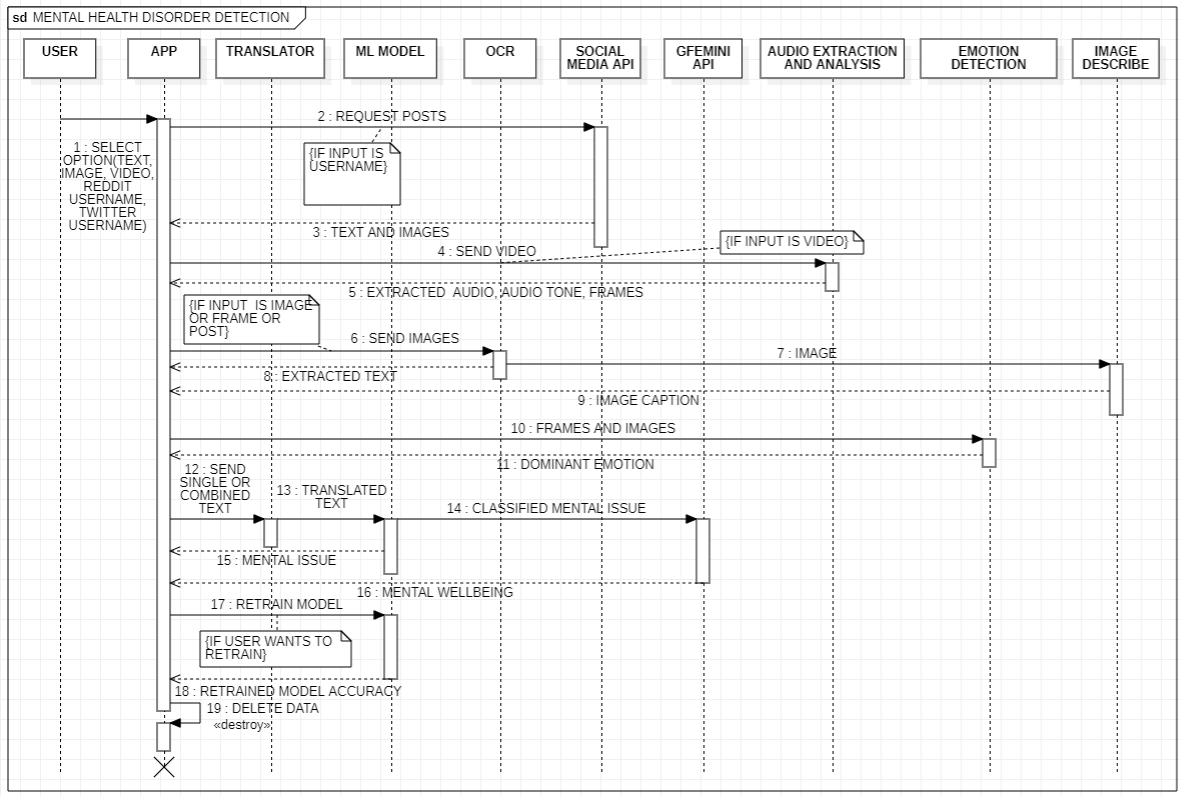
\includegraphics[width=1.0\textwidth]{Images/Sequence Diagram.png}  
    \caption{Sequence Diagram of the Application}
    \label{012i}  % Label for referencing the figure
\end{figure}

\noindent
Below are some screenshots from the web application.

\begin{figure}[h!]  
    \centering
    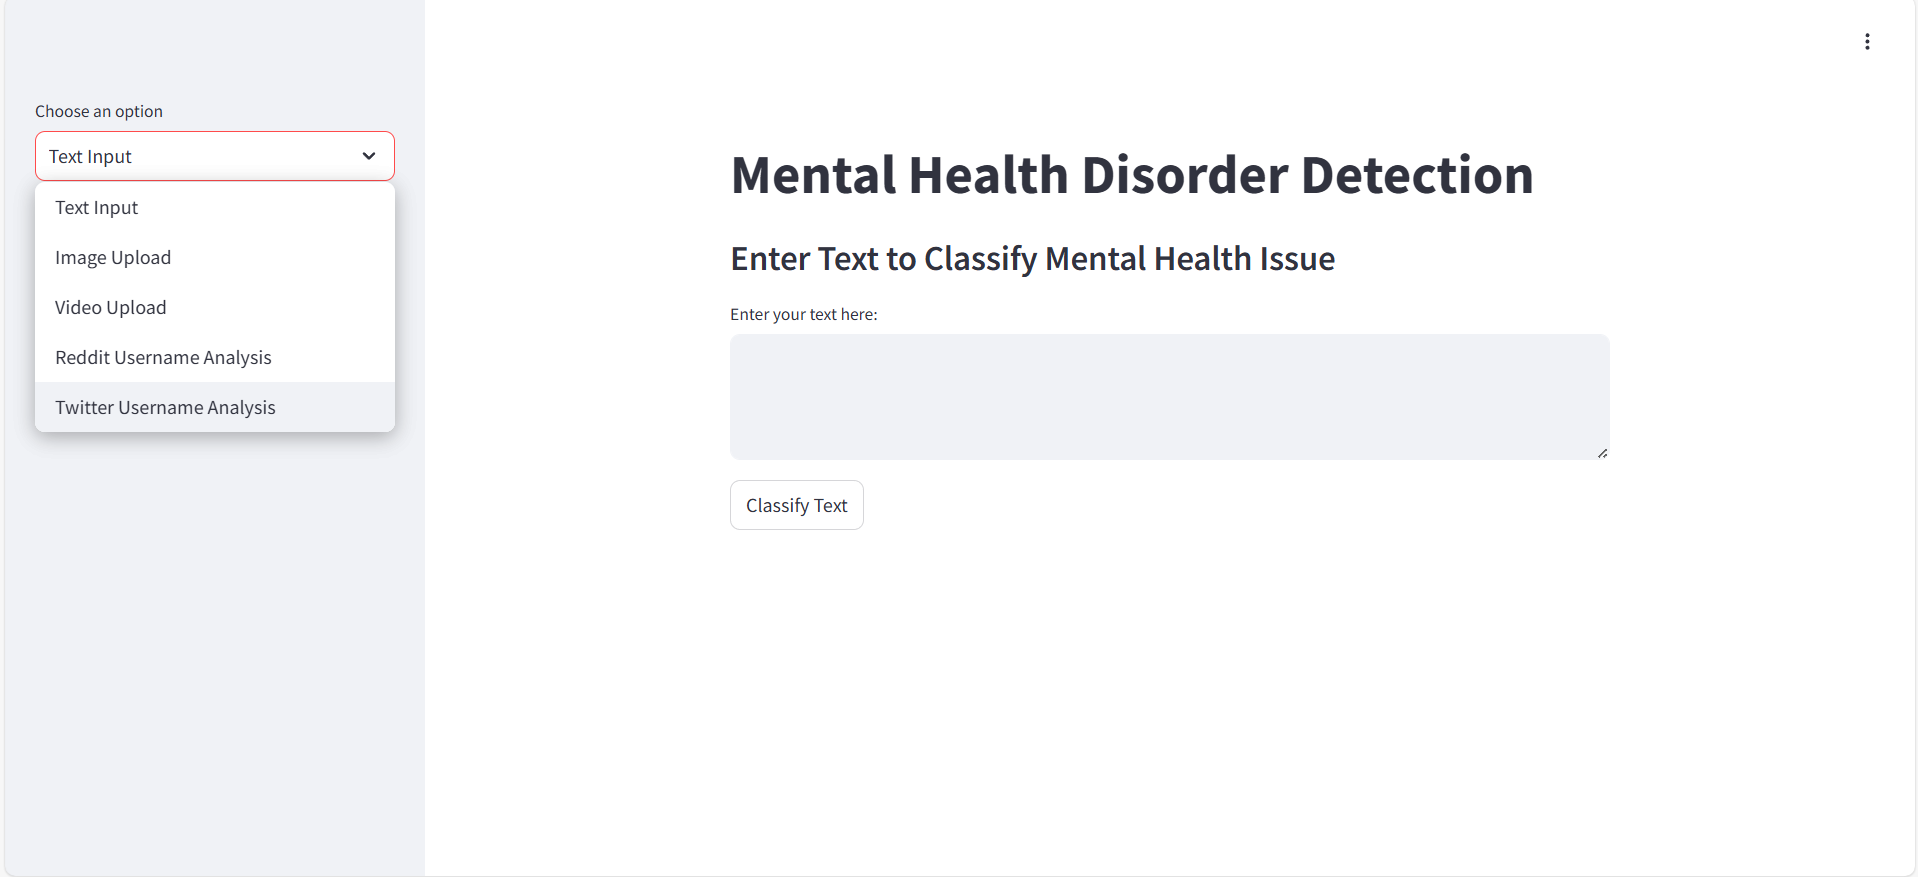
\includegraphics[width=1.0\textwidth]{App Images/01 Interface.png}  
    \caption{Website with all options}
    \label{01i}  % Label for referencing the figure
\end{figure}

\pagebreak

\begin{figure}[h!]  
    \centering
    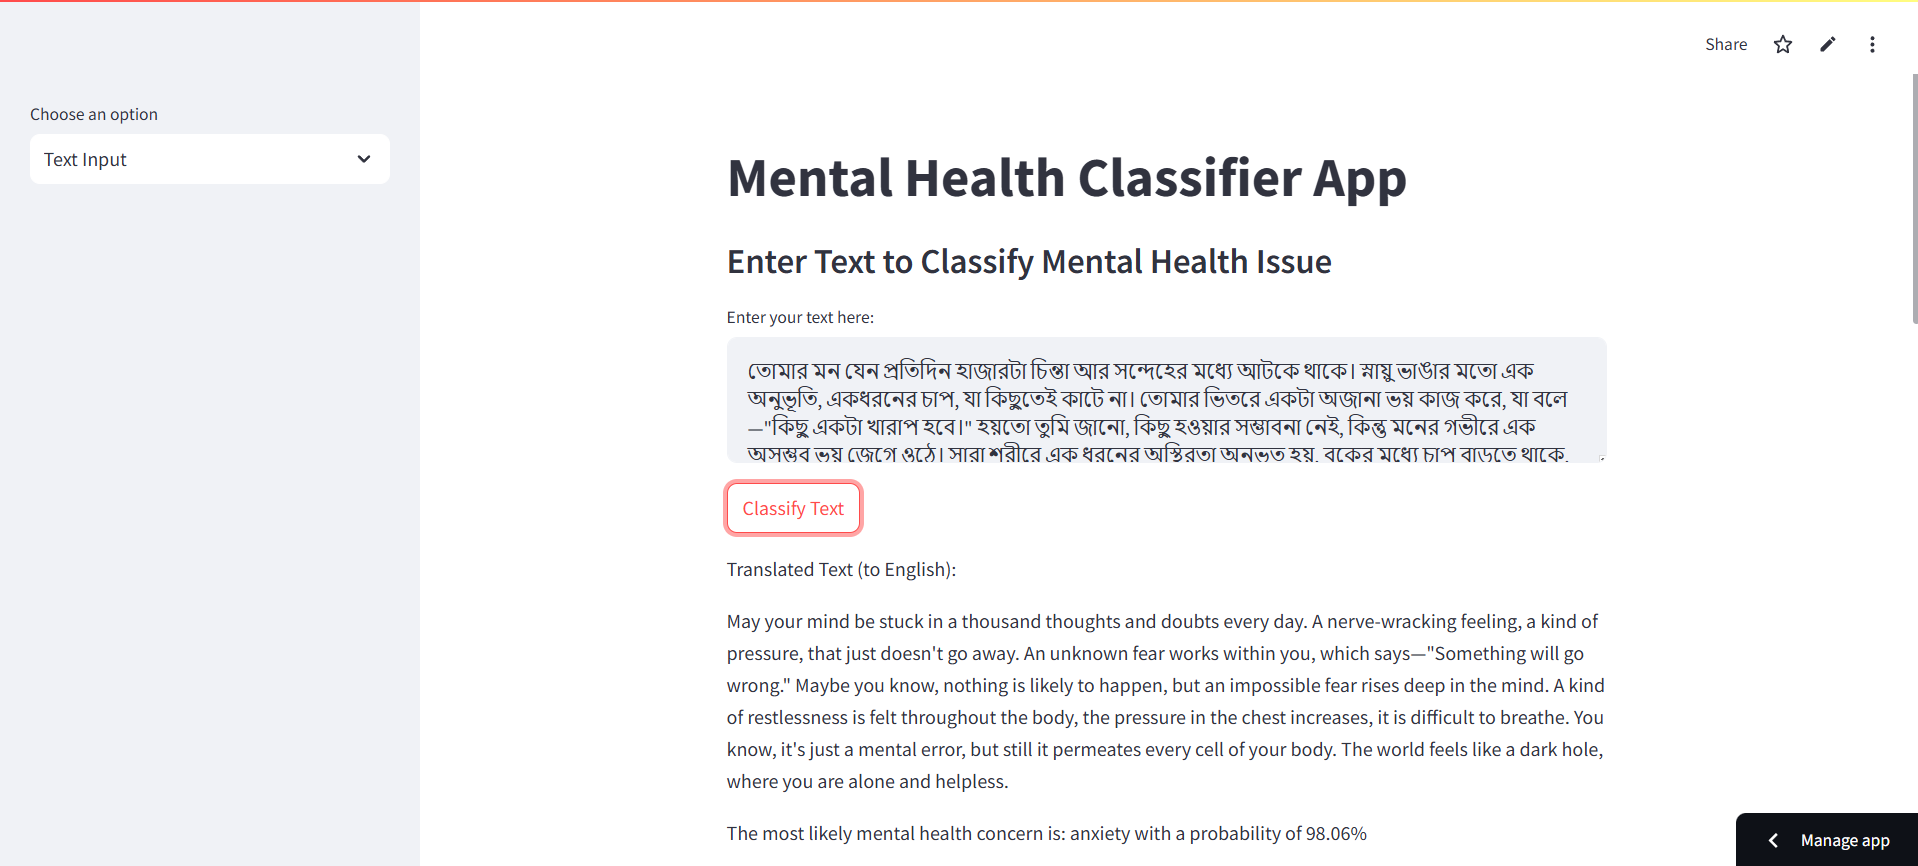
\includegraphics[width=0.8\textwidth]{App Images/02 Interface.png}  
    \caption{Entering Text for classification}
    \label{02i}  % Label for referencing the figure
\end{figure}

\begin{figure}[h!]  
    \centering
    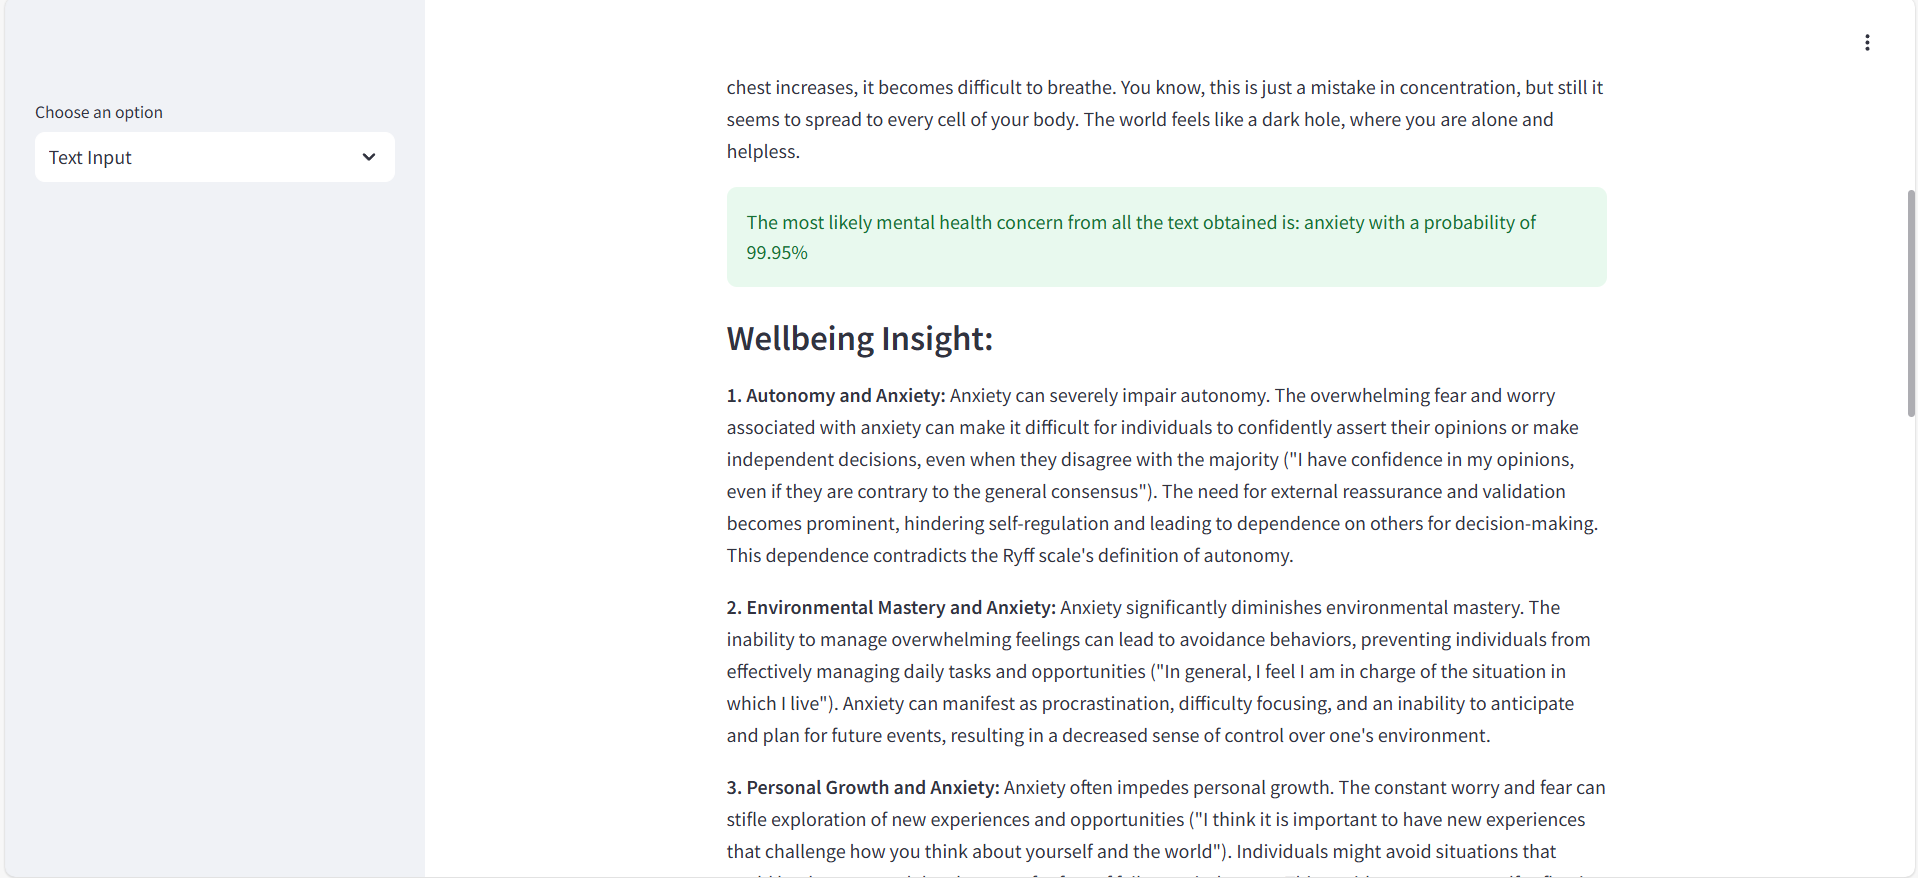
\includegraphics[width=0.8\textwidth]{App Images/03 Interface.png}  
    \caption{Text Classification Result}
    \label{03i}  % Label for referencing the figure
\end{figure}



\begin{figure}[h!]  
    \centering
    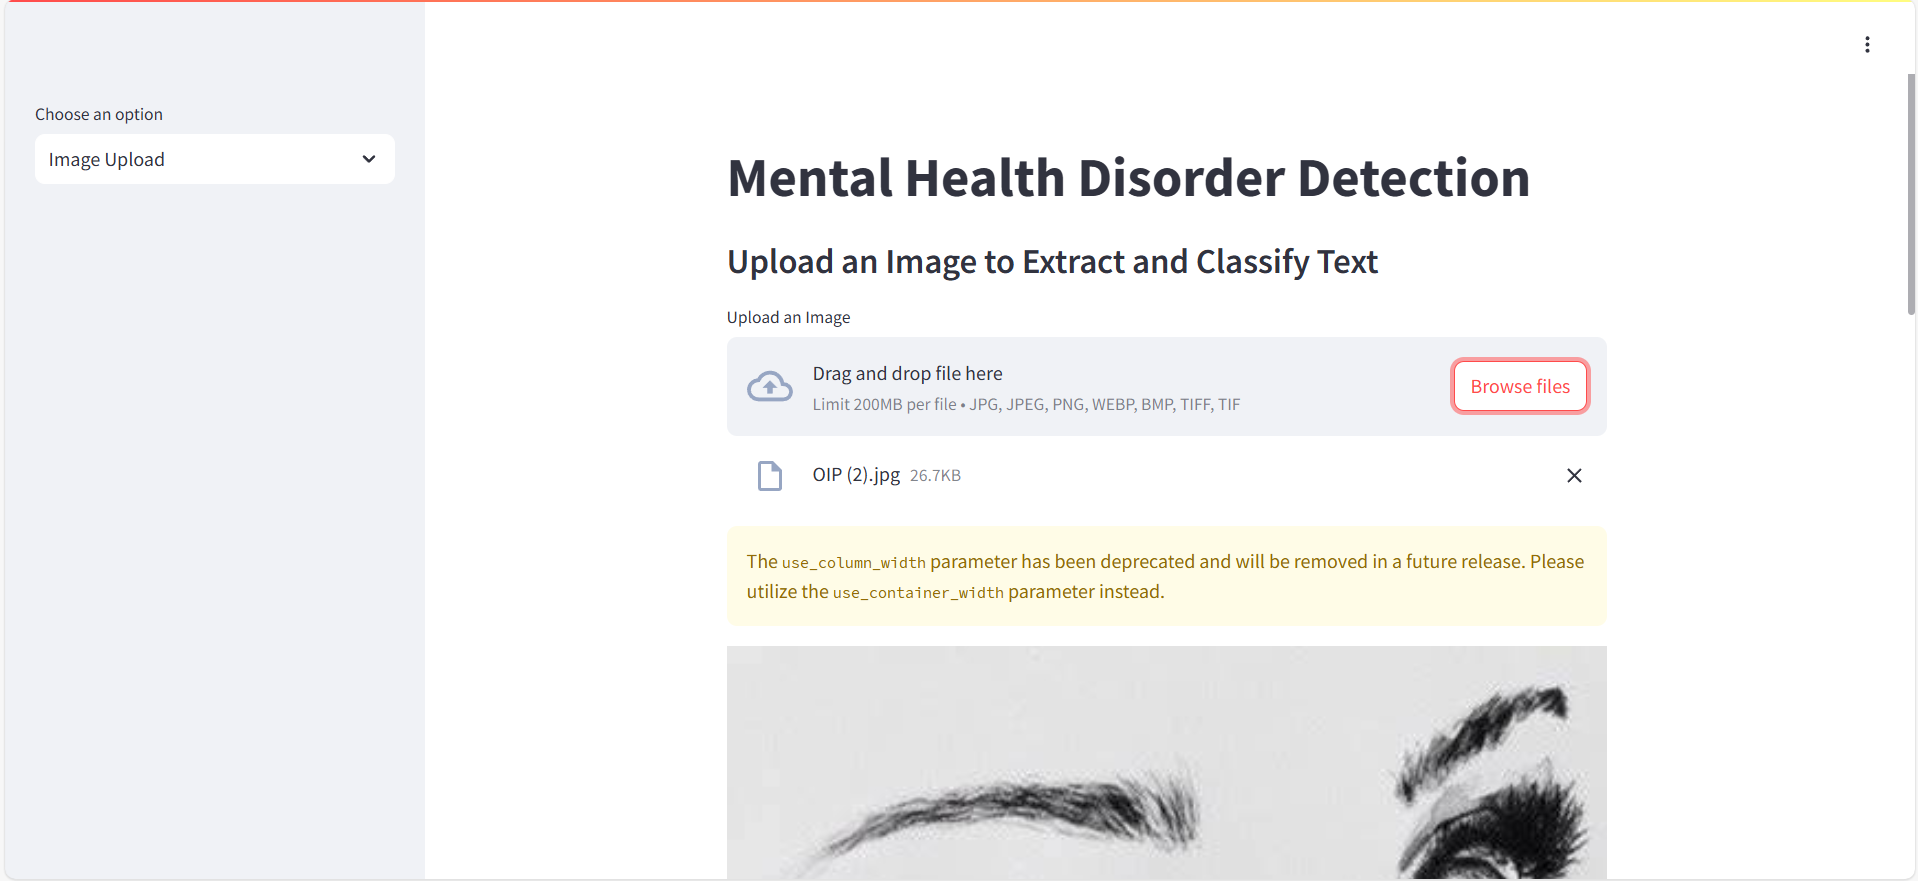
\includegraphics[width=0.8\textwidth]{App Images/04 Interface.png}  
    \caption{Upload Image}
    \label{04i}  % Label for referencing the figure
\end{figure}

\pagebreak

\begin{figure}[h!]  
    \centering
    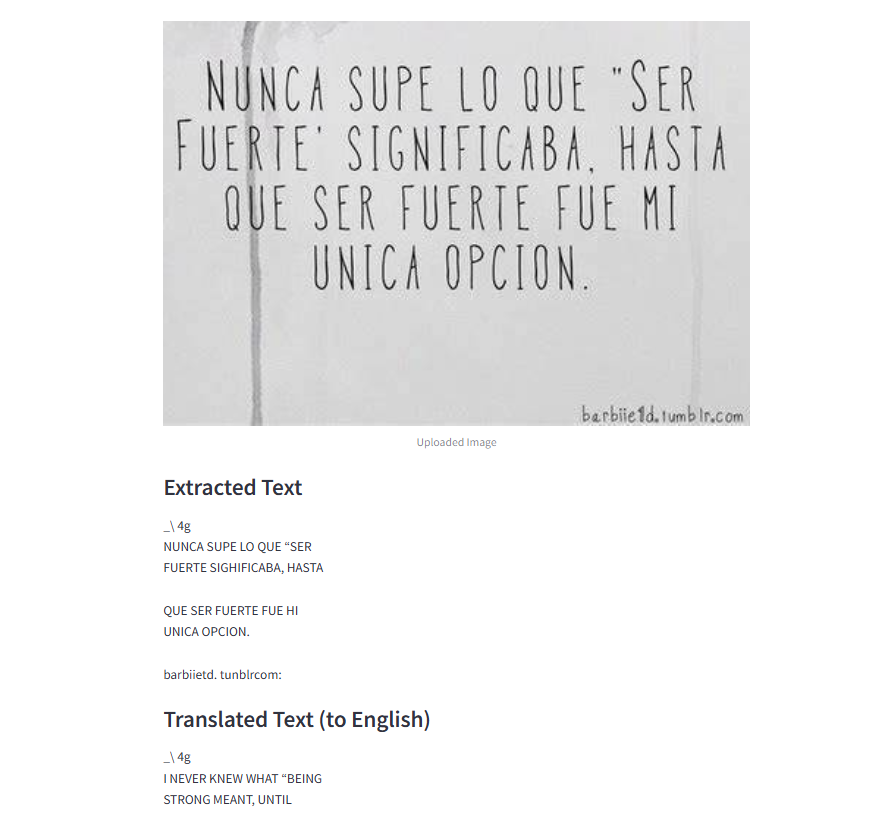
\includegraphics[width=0.8\textwidth]{App Images/05 Interface.png}  
    \caption{Image Classification Result}
    \label{05i}  % Label for referencing the figure
\end{figure}


\begin{figure}[h!]  
    \centering
    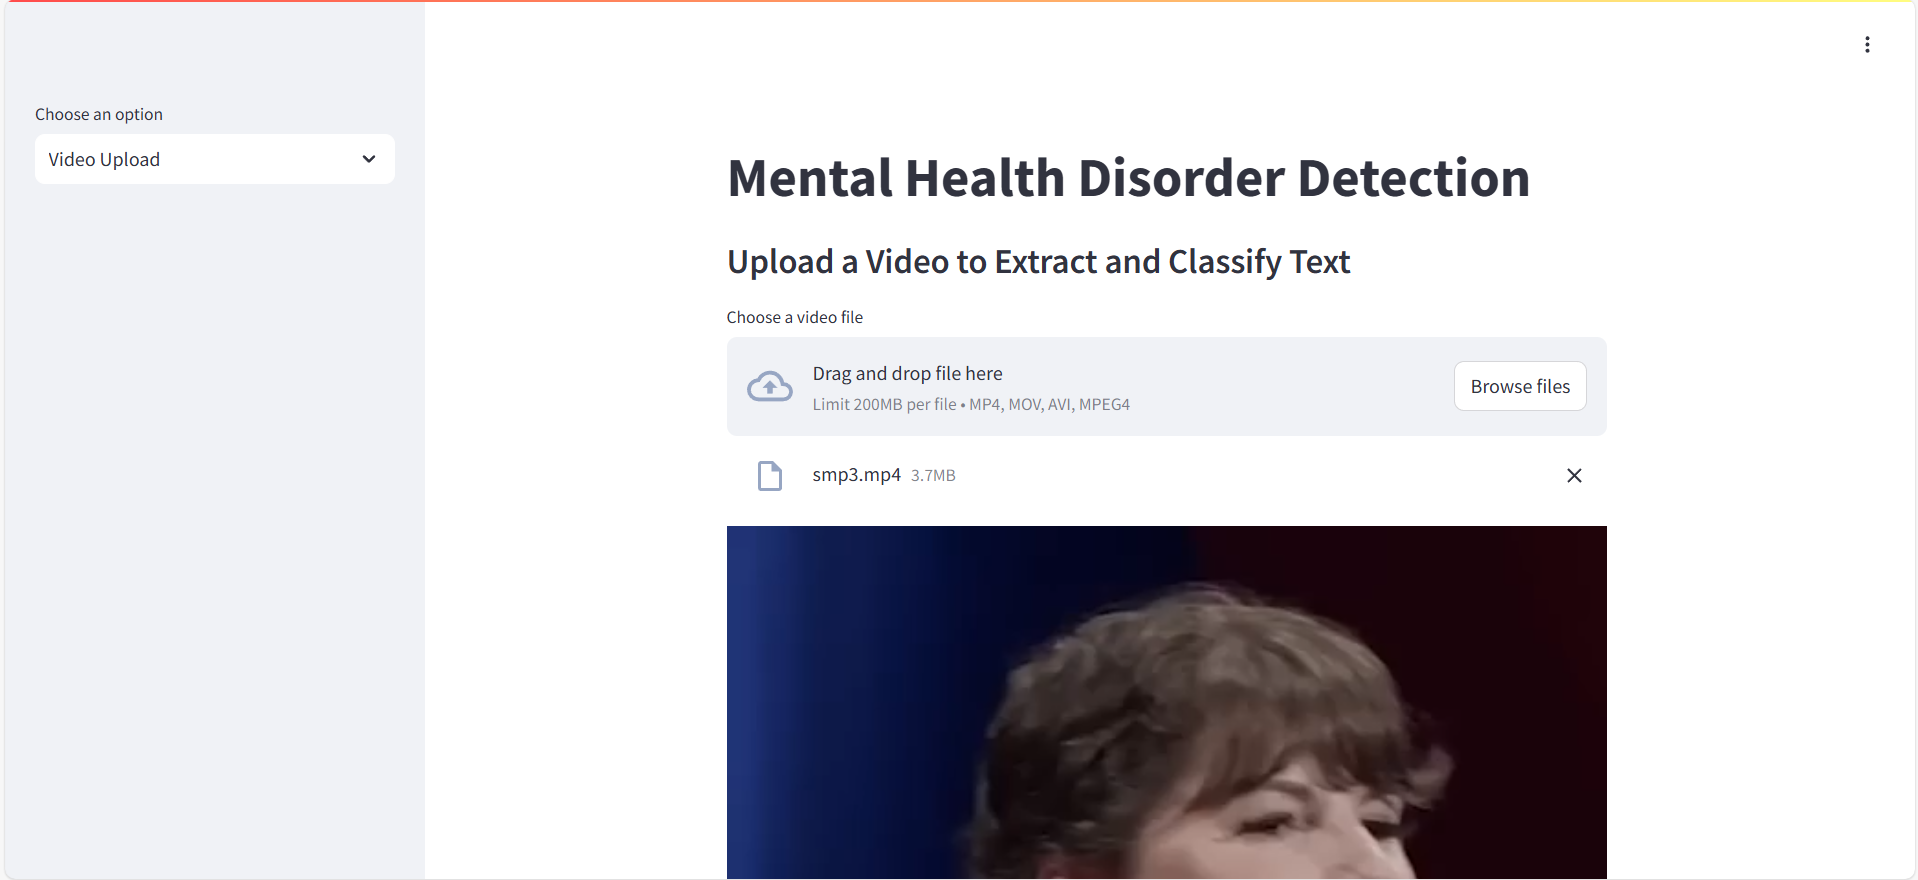
\includegraphics[width=0.8\textwidth]{App Images/12 Interface.png}  
    \caption{Upload Video}
    \label{06i4}  % Label for referencing the figure
\end{figure}

\begin{figure}[h!]  
    \centering
    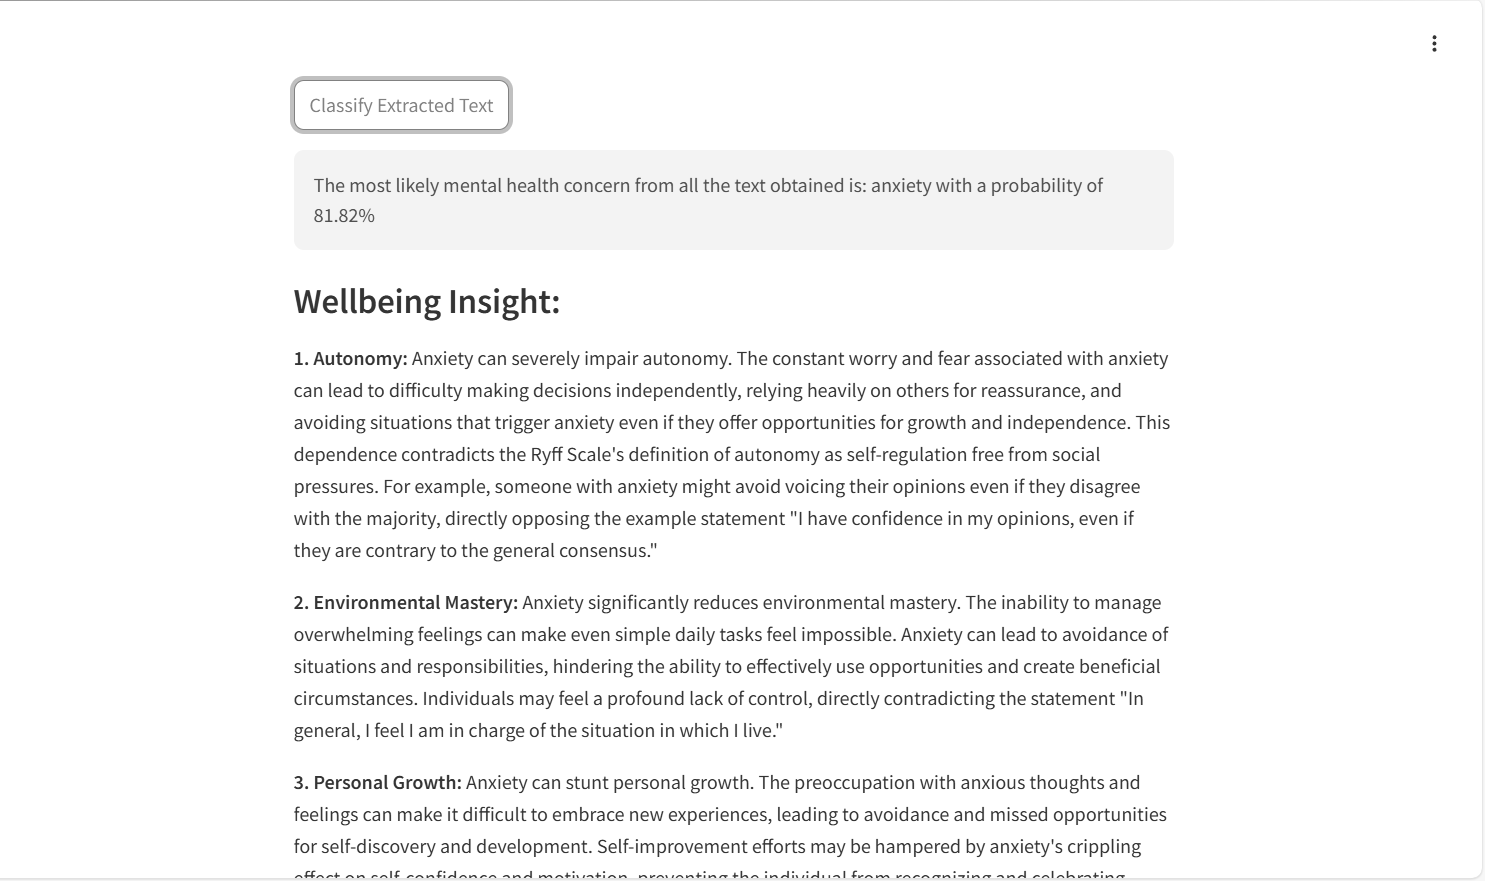
\includegraphics[width=0.8\textwidth]{App Images/13 Interface.png}  
    \caption{Video Classification Result}
    \label{06i}  % Label for referencing the figure
\end{figure}

\pagebreak

\begin{figure}[h!]  
    \centering
    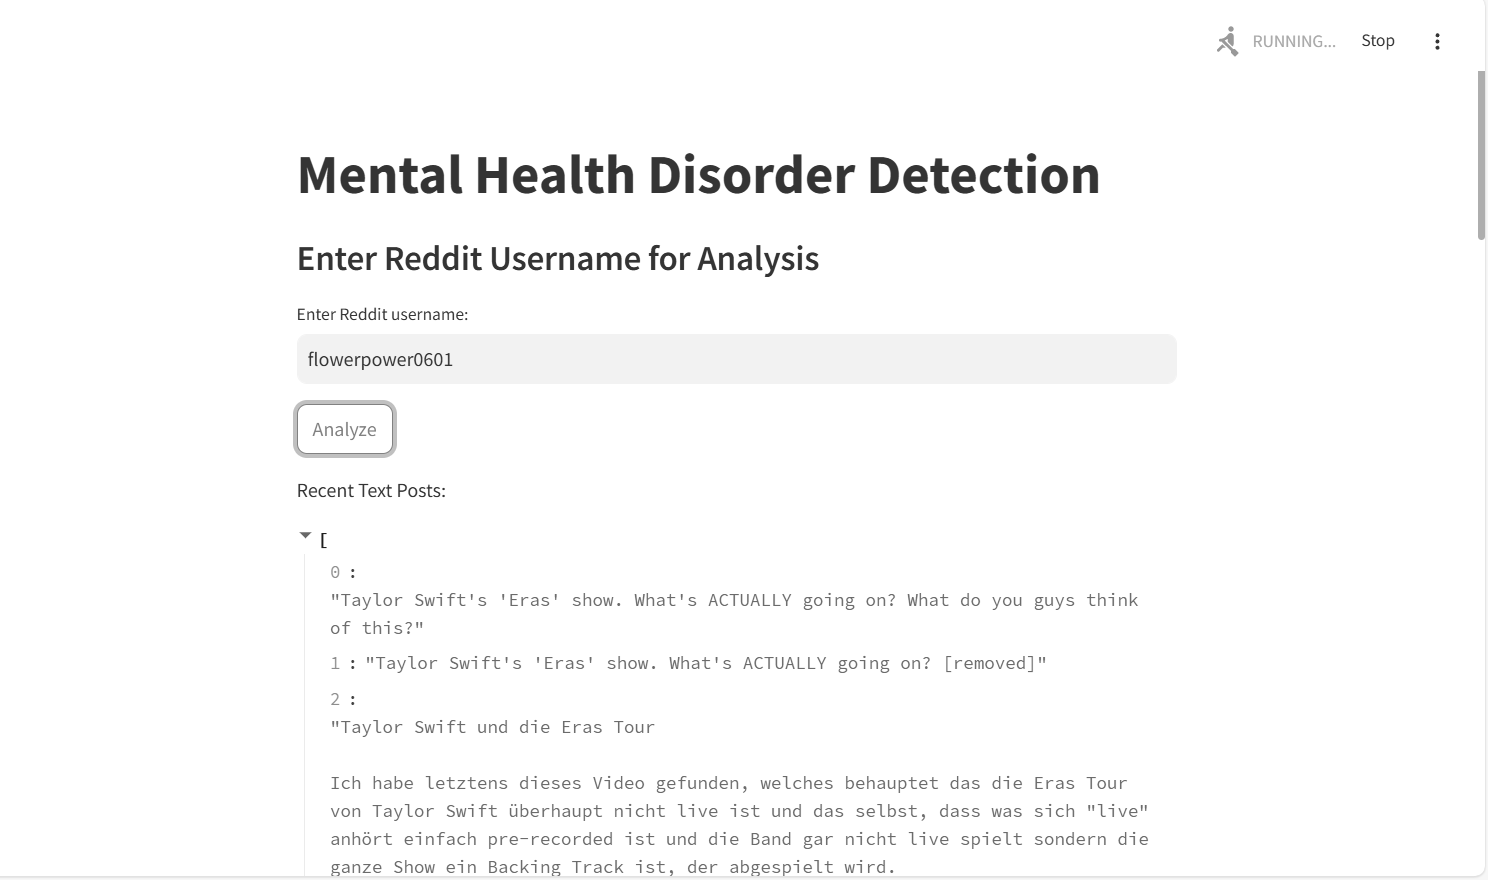
\includegraphics[width=0.8\textwidth]{App Images/06 Interface.png}  
    \caption{Reddit User Analysis}
    \label{07i}  % Label for referencing the figure
\end{figure}

\begin{figure}[h!]  
    \centering
    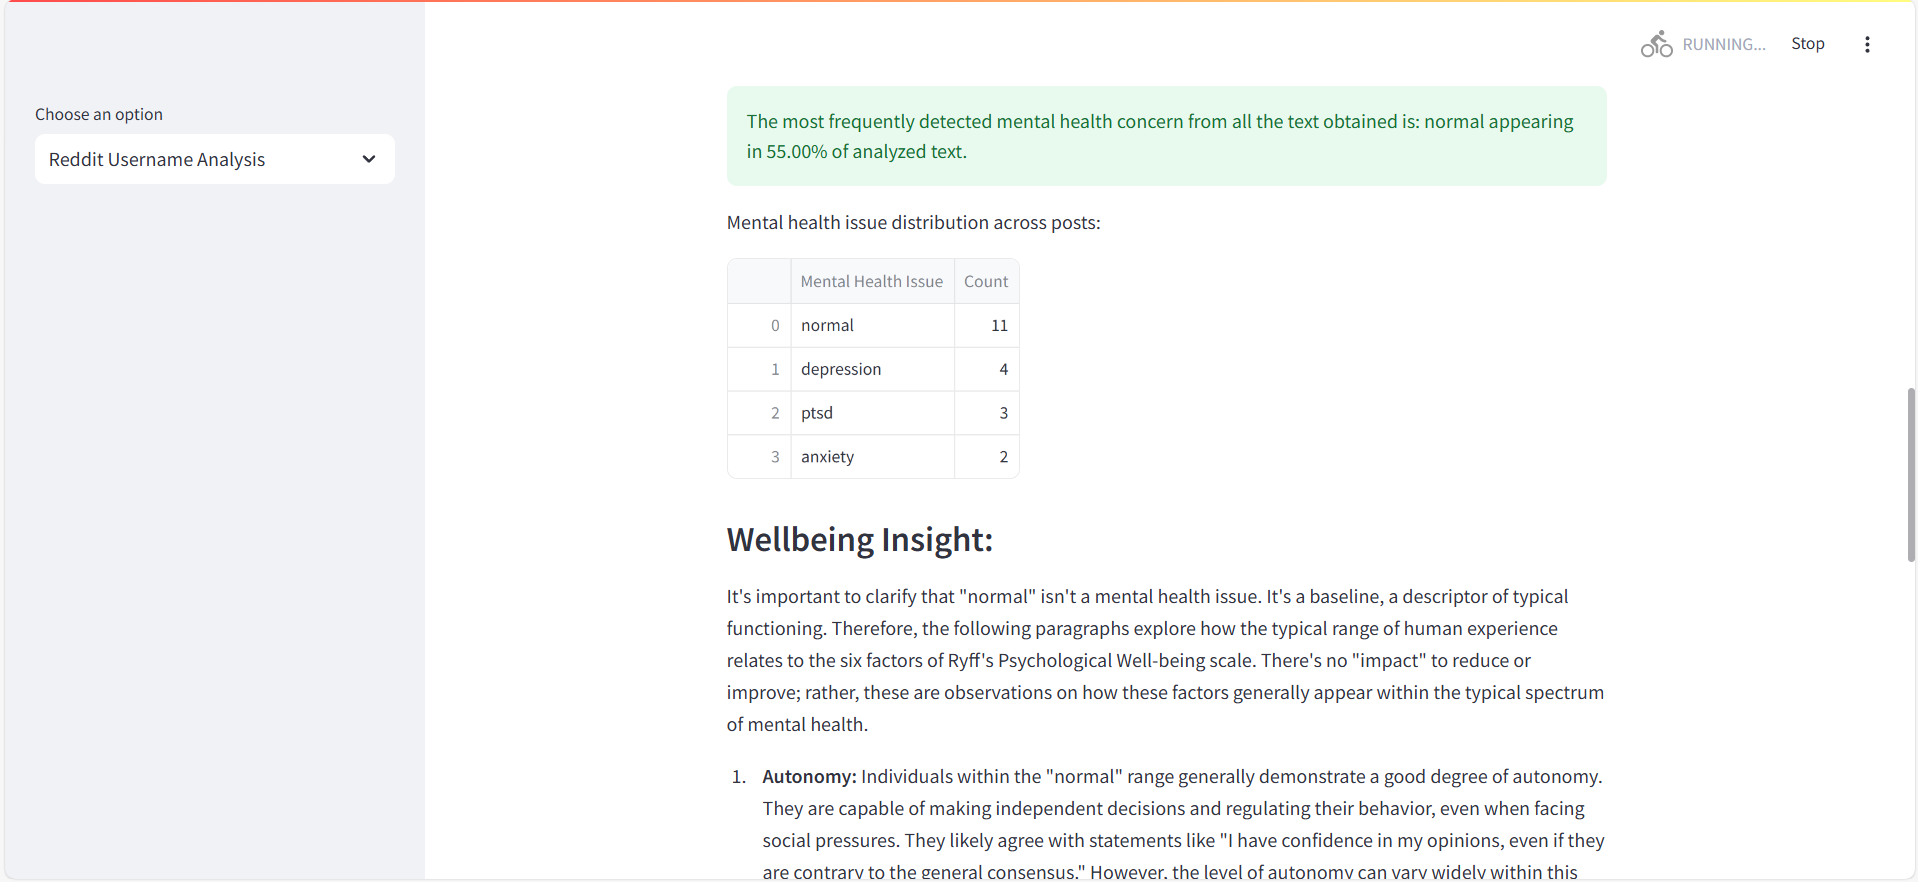
\includegraphics[width=0.8\textwidth]{App Images/07 Interface.png}  
    \caption{Result from Reddit Posts Analysis}
    \label{08i}  % Label for referencing the figure
\end{figure}


\begin{figure}[h!]  
    \centering
    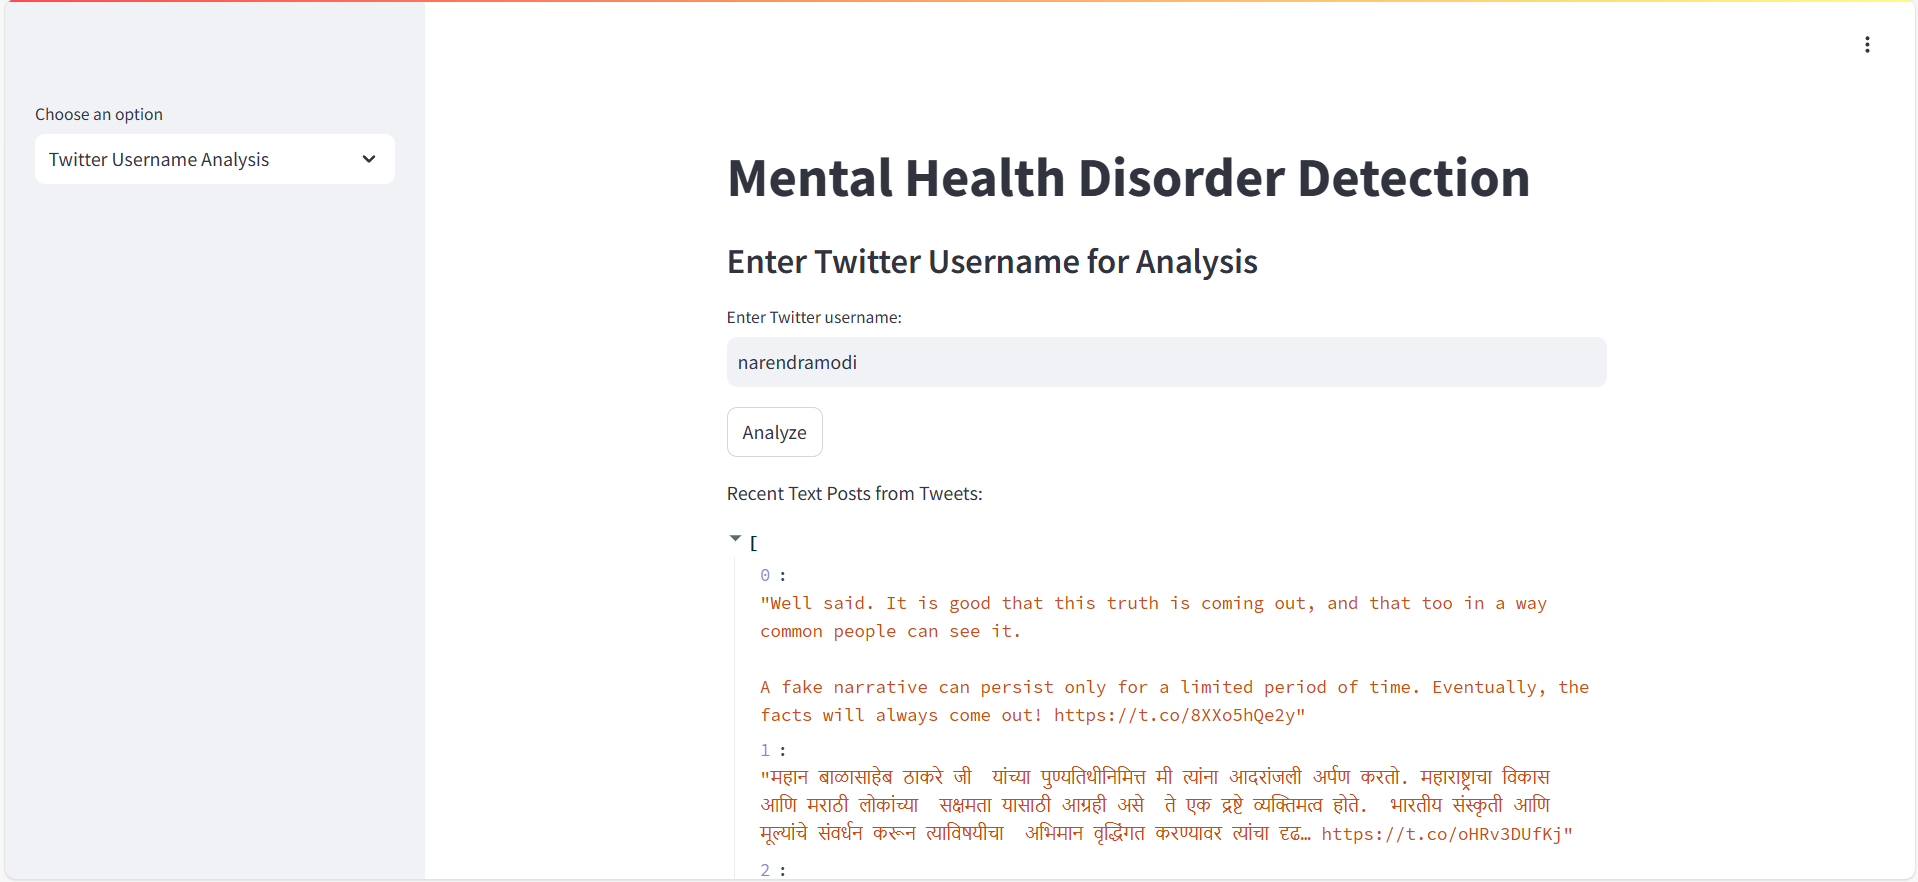
\includegraphics[width=0.8\textwidth]{App Images/08 Interface.png}  
    \caption{Twitter User Analysis}
    \label{09i}  % Label for referencing the figure
\end{figure}

\pagebreak

\begin{figure}[h!]  
    \centering
    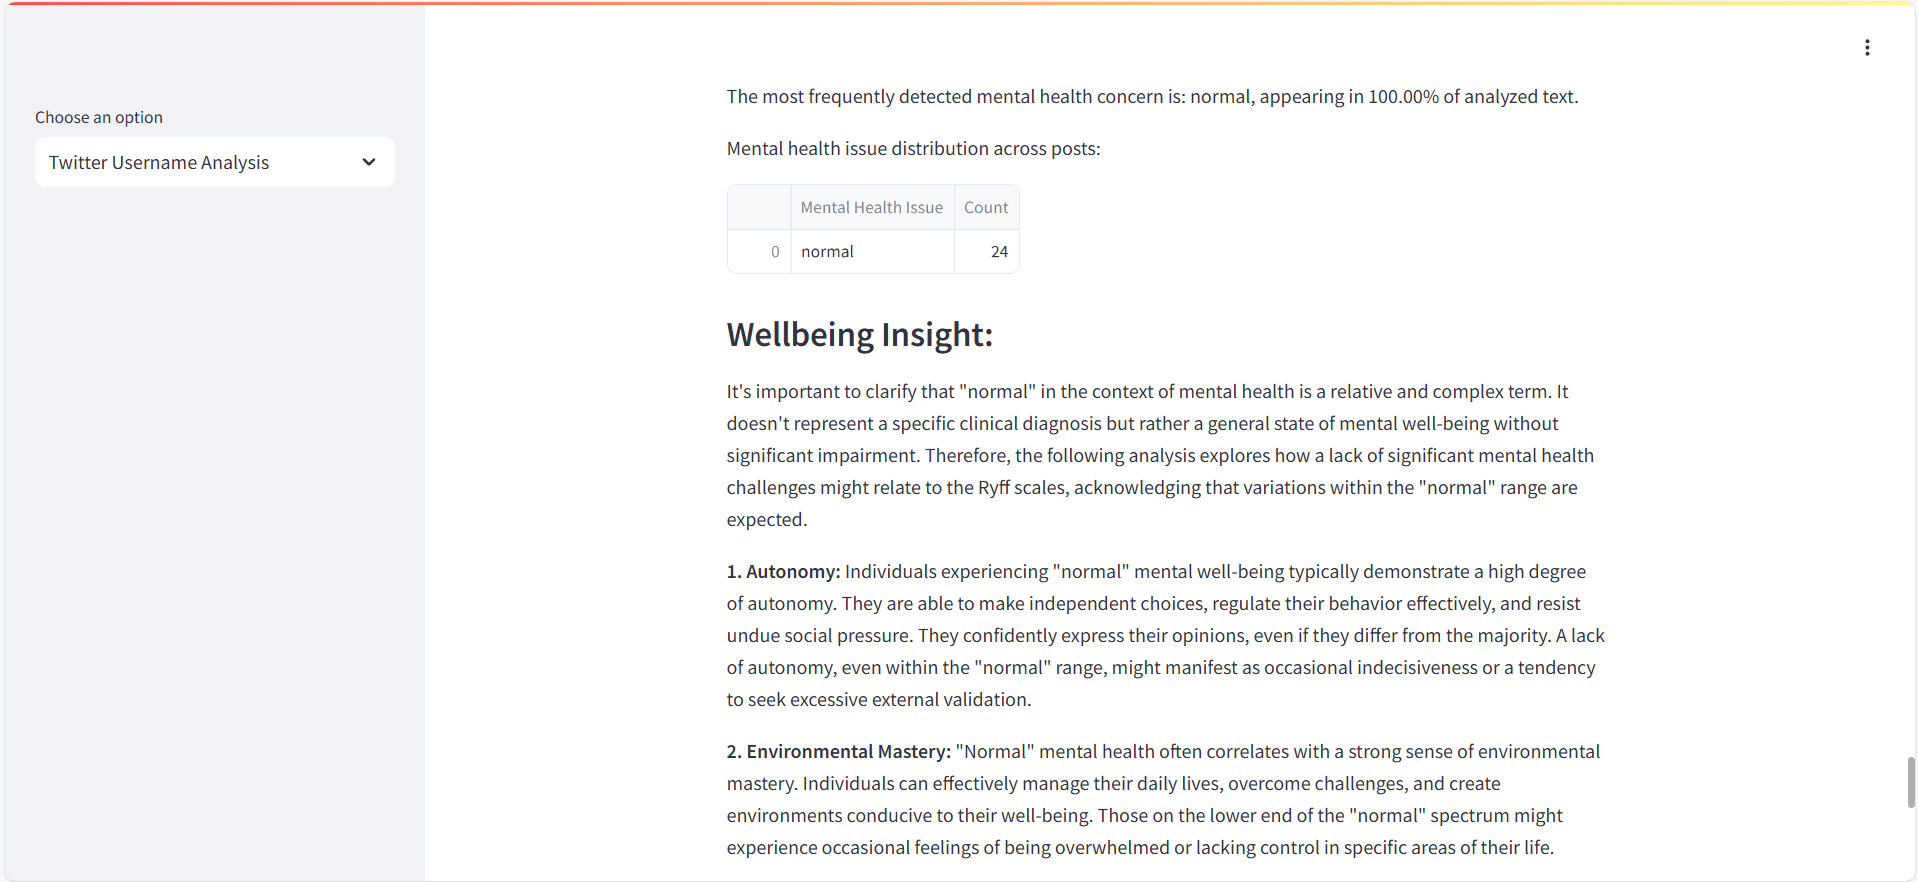
\includegraphics[width=0.9\textwidth]{App Images/10 Interface.png}  
    \caption{Result from Twitter Posts Analysis}
    \label{10i}  % Label for referencing the figure
\end{figure}

% --------- RETRAIN ENSEMBLE MODEL 

\begin{tcolorbox}[colback=gray!5!white, colframe=gray!80!black, boxrule=0.5pt, title=Retraining the Ensemble Model]
    \begin{lstlisting}[language=Python]
def retrain_model():
    # Load Logistic Regression model and vectorizer
    with open('LRmodel.pkl', 'rb') as file:
        lr_model = pickle.load(file)
    with open('LRvectorizer.pkl', 'rb') as file:
        lr_vectorizer = pickle.load(file)

    # Load SVM model and vectorizer
    with open('SVMmodel.pkl', 'rb') as file:
        svm_model = pickle.load(file)
    with open('SVMvectorizer.pkl', 'rb') as file:
        svm_vectorizer = pickle.load(file)

    # Load XGBoost model, vectorizer, and label encoder
    with open('xgb_model.pkl', 'rb') as file:
        xgb_model = pickle.load(file)
    with open('tfidf_vectorizer.pkl', 'rb') as file:
        tfidf_vectorizer = pickle.load(file)
    with open('label_encoder.pkl', 'rb') as file:
        label_encoder = pickle.load(file)

    # Load LSTM model, tokenizer, and label encoder
    lstm_model = load_model('lstm_model.h5')
    with open('LSTM_tokenizer.pkl', 'rb') as file:
        lstm_tokenizer = pickle.load(file)
    \end{lstlisting}
\end{tcolorbox}  
\begin{tcolorbox}[colback=gray!5!white, colframe=gray!80!black, boxrule=0.5pt, title=Retraining the Ensemble Model]
    \begin{lstlisting}[language=Python]      
    # Load Naive Bayes model and vectorizer
    with open('NBmodel.pkl', 'rb') as file:
        nb_model = pickle.load(file)
    with open('NBvectorizer.pkl', 'rb') as file:
        nb_vectorizer = pickle.load(file)

    # Load the test dataset
    data = pd.read_csv('preprocessed_mental_health.csv')

    # Check if 'cleaned_text' column exists
    if 'cleaned_text' not in data.columns:
        raise ValueError("The dataset must have a 'cleaned_text' column.")

    # Remove rows with missing values in 'cleaned_text'
    data.dropna(subset=['cleaned_text'], inplace=True)

    # Split features and target
    X_test = data['cleaned_text']
    y_test = data['mental_health_issue']

    # Encode target labels
    y_test = label_encoder.transform(y_test)

    # Process the text for each model
    X_test_lr = lr_vectorizer.transform(X_test)  # Logistic Regression vectorizer
    X_test_svm = svm_vectorizer.transform(X_test)  # SVM vectorizer
    X_test_xgb = tfidf_vectorizer.transform(X_test)  # XGBoost vectorizer
    X_test_nb = nb_vectorizer.transform(X_test)  # Naive Bayes vectorizer
    X_test_lstm = lstm_tokenizer.texts_to_sequences(X_test)  # LSTM tokenizer

    # Pad sequences for LSTM
    X_test_lstm = pad_sequences(X_test_lstm, maxlen=100, padding='post', truncating='post')

    # Get predictions from the base models
    lr_predictions_proba = lr_model.predict_proba(X_test_lr)  # Logistic Regression probabilities
    svm_predictions_proba = svm_model.predict_proba(X_test_svm)  # SVM probabilities
    \end{lstlisting}
\end{tcolorbox}
\begin{tcolorbox}[colback=gray!5!white, colframe=gray!80!black, boxrule=0.5pt, title=Retraining the Ensemble Model]
    \begin{lstlisting}[language=Python]
    xgb_predictions_proba = xgb_model.predict_proba(X_test_xgb)  # XGBoost probabilities
    nb_predictions_proba = nb_model.predict_proba(X_test_nb)  # Naive Bayes probabilities
    lstm_predictions_proba = lstm_model.predict(X_test_lstm)  # LSTM probabilities

    # Stack the predictions of all models to create the feature matrix for the meta-learner
    stacked_features = np.hstack((lr_predictions_proba, svm_predictions_proba, xgb_predictions_proba, nb_predictions_proba, lstm_predictions_proba))

    # Define the Logistic Regression model for the meta-learner
    meta_learner_lr = LogisticRegression(max_iter=5000)
    
    # Train the Logistic Regression meta-learner on the full dataset
    meta_learner_lr.fit(stacked_features, y_test)
    
    # Save the trained Logistic Regression meta-learner
    with open('meta_learner_lr.pkl', 'wb') as file:
        pickle.dump(meta_learner_lr, file)
    
    # Predict using the Logistic Regression meta-learner
    final_predictions_lr = meta_learner_lr.predict(stacked_features)
    
    # Evaluate the Logistic Regression ensemble model
    accuracy_lr = accuracy_score(y_test, final_predictions_lr)

    return meta_learner_lr, accuracy_lr
\end{lstlisting}
\end{tcolorbox}

\noindent
The above function, \texttt{retrain\_model}, is designed to retrain an ensemble learning model (similar for adding transformer by loading the transformer files) using an updated dataset. Initially, it loads multiple base models (Logistic Regression, SVM, XGBoost, Naive Bayes, and LSTM) along with their respective vectorizers, tokenizers, and label encoder from previously saved pickle files. The function then loads and preprocesses the updated dataset, ensuring it contains the necessary text column (\texttt{cleaned\_text}) and splitting it into features (\texttt{X\_test}) and target labels (\texttt{y\_test}). The target labels are encoded using the label encoder, while the text features are transformed using the corresponding vectorizers or tokenizers for each model. Predictions from each model are then collected, stacked together, and used to retrain the meta-learner (RandomForestClassifier). Once trained, the meta-learner is saved for future use.

% --------- ENSEMBLE MODEL


\pagebreak

\begin{figure}[h!]  
    \centering
    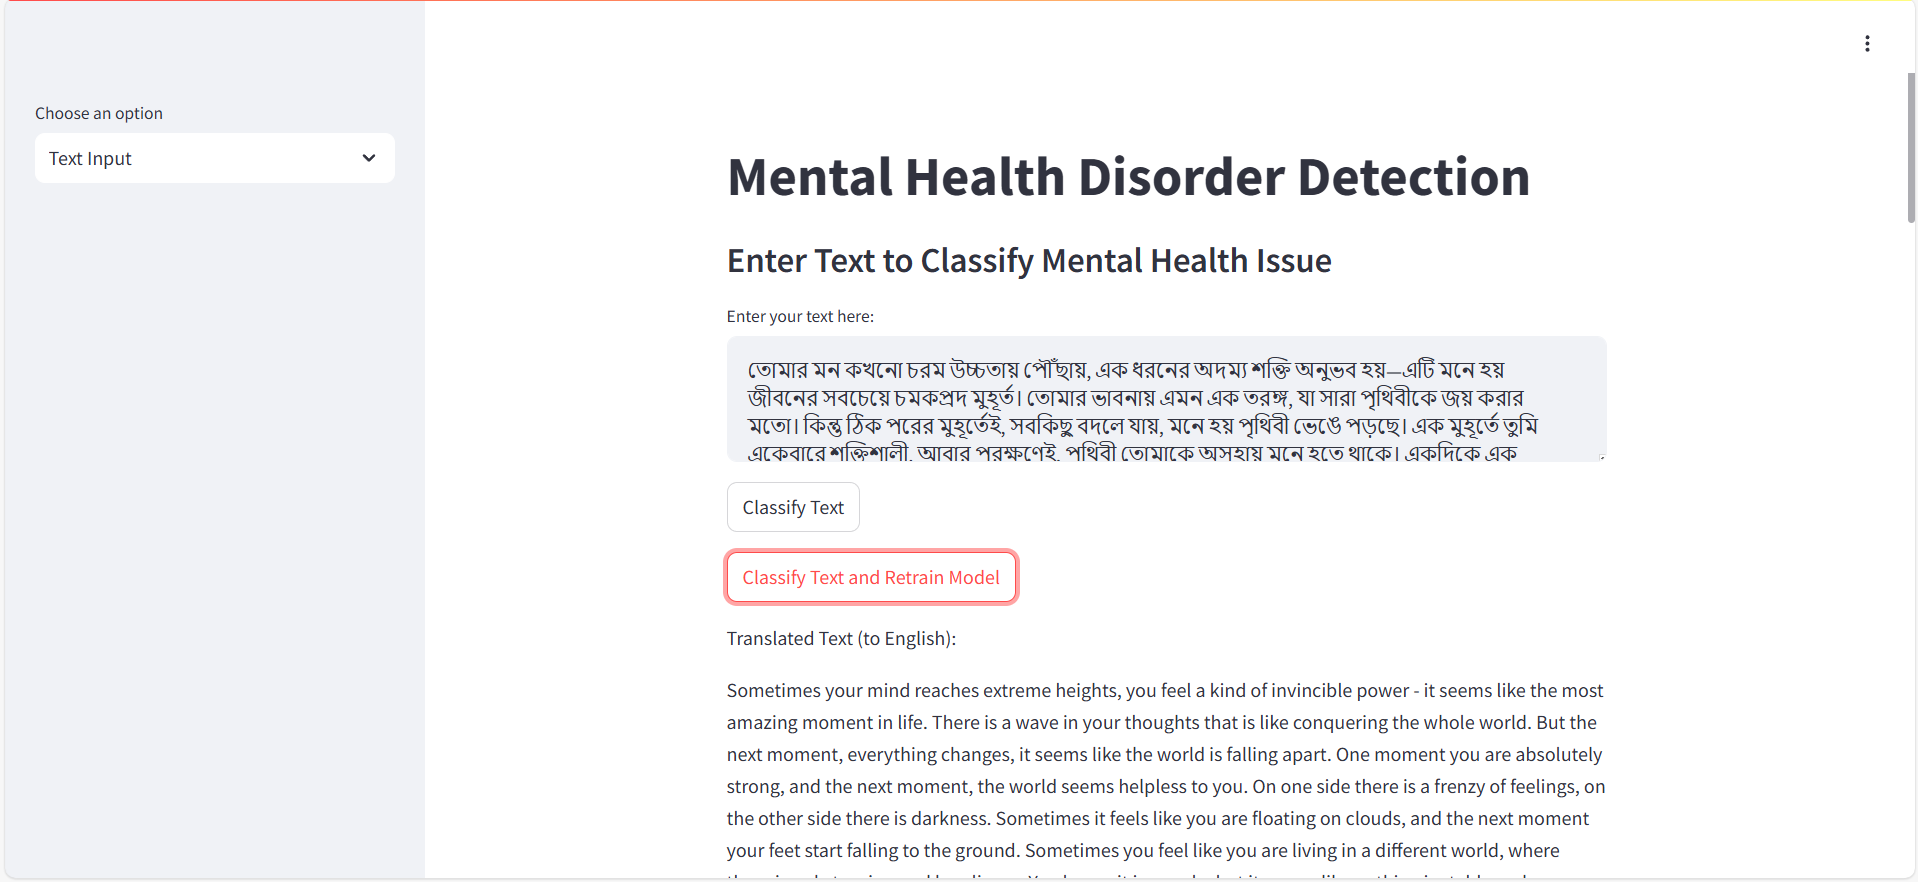
\includegraphics[width=0.8\textwidth]{App Images/14 Interface.png}  
    \caption{Text Classification and Retrain Model}
    \label{101i}  % Label for referencing the figure
\end{figure}

\begin{figure}[h!]  
    \centering
    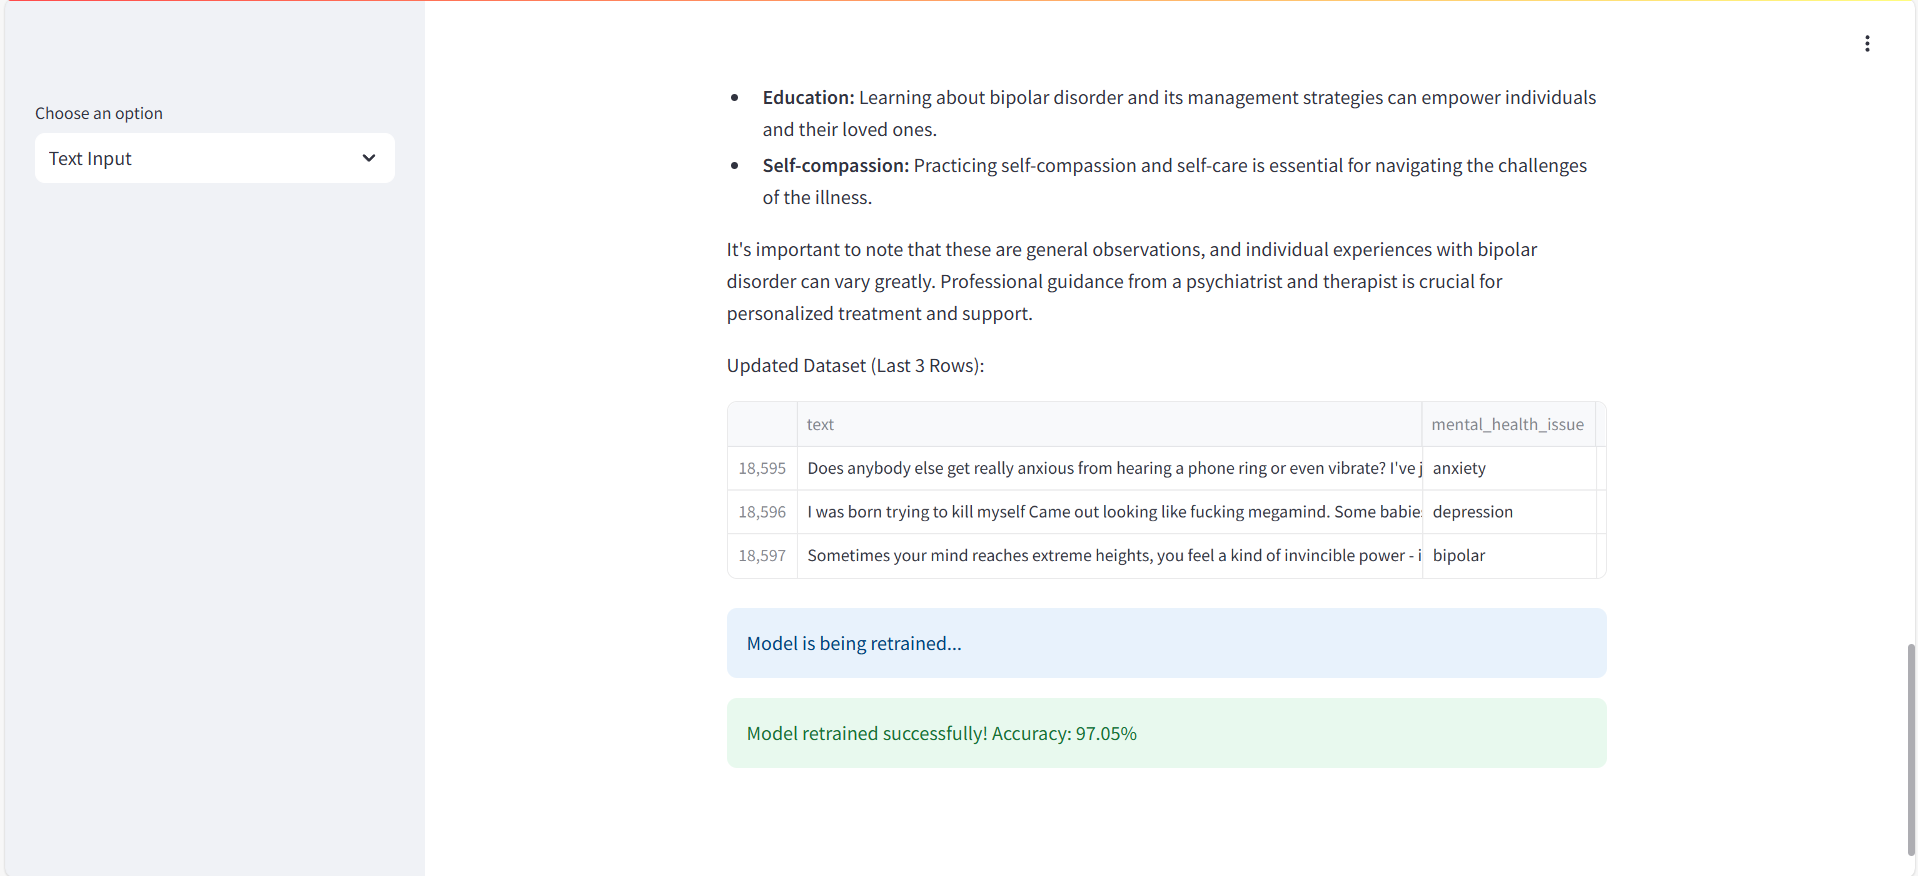
\includegraphics[width=0.8\textwidth]{App Images/15 Interface.png}  
    \caption{Result from Text Classification and Model Retraining}
    \label{102i}  % Label for referencing the figure
\end{figure}

\begin{figure}[h!]  
    \centering
    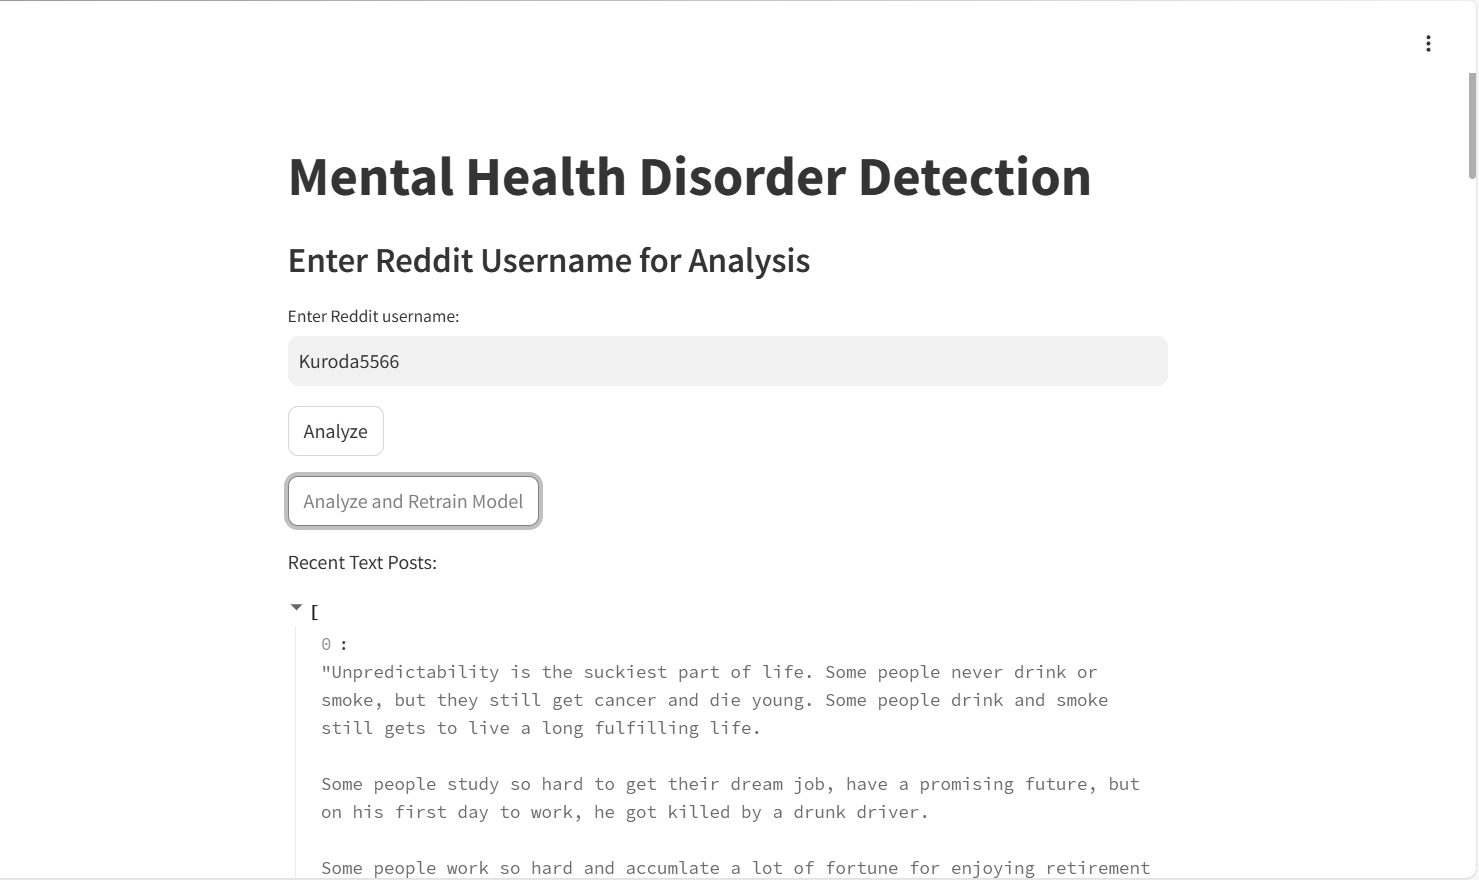
\includegraphics[width=0.8\textwidth]{App Images/16 Interface.png}  
    \caption{Reddit Analysis with Model Retraining}
    \label{10i}  % Label for referencing the figure
\end{figure}

\pagebreak

\begin{figure}[h!]  
    \centering
    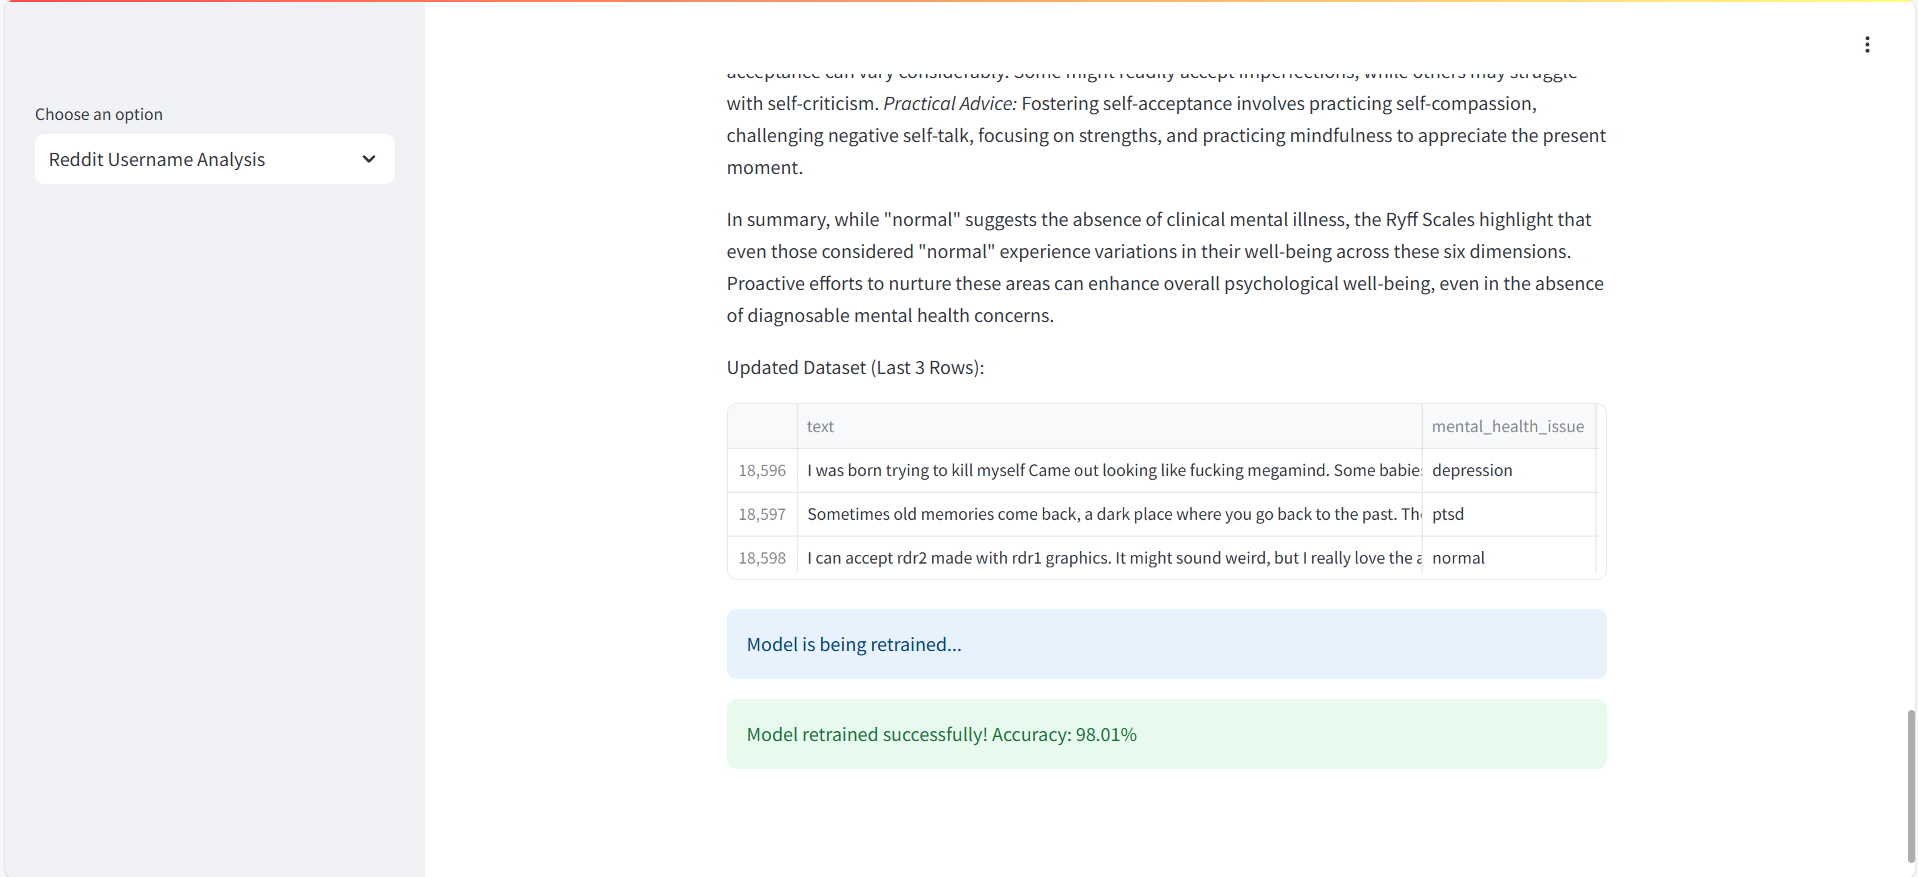
\includegraphics[width=0.9\textwidth]{App Images/17 Interface.png}  
    \caption{Result from Reddit Analysis and Model Retraining}
    \label{10i}  % Label for referencing the figure
\end{figure}


\begin{tcolorbox}[colback=gray!5!white, colframe=gray!80!black, boxrule=0.5pt, title=Emotion Analysis and Mental Health Insights]
    \begin{lstlisting}[language=Python]
def detect_emotions_from_frame(frame):
    try:
        # Use DeepFace to analyze emotions
        result = DeepFace.analyze(frame, actions=['emotion'], enforce_detection=False)
        return result[0]['dominant_emotion']
    except Exception as e:
        print(f"No expression or error detecting emotion: {e}")
        return None

def analyze_emotions_from_frames(frames):
    # Initialize an emotion counts dictionary
    emotion_counts = {'happy': 0, 'sad': 0, 'angry': 0, 'disgust': 0, 'fear': 0, 'surprise': 0, 'neutral': 0}
    frame_emotions = []

    for idx, frame in enumerate(frames):
        # Detect emotions from the current frame
        emotion = detect_emotions_from_frame(frame)
        if emotion:
            frame_emotions.append(emotion)
            if emotion in emotion_counts:
                emotion_counts[emotion] += 1

    return emotion_counts, frame_emotions
\end{lstlisting}
\end{tcolorbox}
\begin{tcolorbox}[colback=gray!5!white, colframe=gray!80!black, boxrule=0.5pt, title=Emotion Analysis and Mental Health Insights]
    \begin{lstlisting}[language=Python]
def display_emotion_summary(emotion_counts):
    # Convert the emotion counts to a DataFrame for display
    emotion_df = pd.DataFrame(list(emotion_counts.items()), columns=['Emotion', 'Count'])
    st.write("Emotion Analysis Summary:")
    st.table(emotion_df)
    return max(emotion_counts, key=emotion_counts.get)

def analyze_with_gemini(dominant_emotion, emotion_counts):
    try:
        # Start a chat session with the Gemini API
        chat_session = gemini_model.start_chat(history=[])

        # Summarize emotion counts for the prompt
        emotion_summary = ", ".join([f"{emotion}: {count}" for emotion, count in emotion_counts.items()])
        # Create a prompt for the Gemini API
        prompt = (
            f"The detected dominant emotion is '{dominant_emotion}'. "
            f"{emotion_summary}. Based on this information, analyze the potential implications for mental health "
            f"conditions such as depression, anxiety, PTSD, or bipolar disorder. Provide actionable insights in three lines."
        )

        # Send the prompt and get a response
        response = chat_session.send_message(prompt)
        st.write(response.text)
    except Exception as e:
        print(f"Error in Gemini API call: {e}")
        return "An error occurred while communicating with the Gemini API. Please try again later."
    \end{lstlisting}
\end{tcolorbox}

\noindent
The functions in the code work together to analyze emotions from video frames. The detect\_emotions\_from\_frame(frame) function utilizes the DeepFace library to detect the dominant emotion in a given video frame, returning None if no emotion is detected or an error occurs. The analyze\_emotions\_from\_frames(frames) function iterates over multiple video frames, applying detect\_emotions\_from\_frame to each and counting the frequency of detected emotions in a dictionary. The display\_emotion\_summary(emotion\_counts) function uses Streamlit to display a summary of detected emotions in a table format and identifies the dominant emotion with the highest count. Lastly, analyze\_with\_gemini(dominant\_emotion, emotion\_counts) communicates with the Gemini API by preparing a prompt based on the emotion analysis, sending it to the API, and displaying the response in Streamlit, while also handling any potential errors during the API interaction.


\vspace{1em}
\noindent
The DeepFace Python module is a comprehensive framework for facial recognition and facial attribute analysis using deep learning. It provides a high-level interface to process and analyze facial data through a variety of pre-trained deep learning models. The module is designed to make facial recognition, emotion detection, age estimation, and gender detection straightforward by abstracting the complexities of deep learning. DeepFace supports multiple state-of-the-art face recognition models, including VGG-Face, Google FaceNet, OpenFace, Facebook DeepFace, and Dlib. Users can choose any of these models depending on their specific requirements. It also integrates with various facial attribute models for emotion analysis, enabling it to classify emotions such as happiness, sadness, anger, and more. The module uses TensorFlow and Keras as its backend frameworks to run deep learning operations efficiently. At its core, DeepFace operates by detecting and aligning faces in an image using a pre-trained facial detector, ensuring consistent positioning before feeding the face into recognition or analysis pipelines. This preprocessing step is critical because it eliminates variability caused by head tilt, lighting, and facial orientation. For emotion detection specifically, DeepFace uses a softmax classifier at the final layer of its models to predict probabilities for different emotions. DeepFace is also known for its flexibility and simplicity. Users can invoke facial analysis or recognition with a single line of code. Additionally, the module includes an \textbf{analyze} function for emotion, age, and gender detection, as well as a \textbf{verify} function to compare two images for identity matching. It also allows users to toggle between facial detectors, including OpenCV, SSD, and MTCNN, depending on their hardware and processing needs. The module emphasizes usability with optional parameters for tuning accuracy, speed, and error handling. For example, users can enable or disable facial detection enforcement, which is useful in scenarios where non-human faces or partial occlusions are present. The ability to batch process multiple images and integrate seamlessly with large datasets makes DeepFace a preferred choice for production-level applications. Overall, DeepFace abstracts the complexities of implementing deep learning models for facial analysis, providing a user-friendly and powerful tool for a variety of facial recognition and emotion detection tasks.

\vspace{1em}

\noindent
In a mental health disorder detection application, DeepFace plays a pivotal role in extracting facial expressions from images and videos, which can be critical for assessing emotional states and providing insights into potential mental health concerns. The module leverages deep learning models trained to recognize a wide array of facial expressions, such as happiness, sadness, anger, surprise, fear, and disgust. These expressions are vital indicators of a person’s emotional state, which, when analyzed over time, can offer valuable clues about their mental health. DeepFace first processes the input image or video by detecting faces through a facial recognition model, ensuring that only human faces are analyzed. Once faces are detected, the module aligns and normalizes the images to account for variations in lighting, angles, and head positions, ensuring that the analysis remains accurate regardless of how the subject is positioned or oriented. DeepFace's emotion detection model then works by analyzing the subtle changes in facial muscle movements that correspond to different emotional expressions. For instance, a furrowed brow and tight lips may indicate anger, while a smiling face may suggest happiness. These expressions are captured and classified using convolutional neural networks (CNNs), which are adept at identifying patterns in visual data. DeepFace outputs these emotions as probability scores, allowing the application to interpret the likelihood of each emotion being present in a given frame. In a video context, the module processes each frame sequentially, enabling the tracking of emotional transitions over time, which is particularly valuable in detecting mood fluctuations or episodes commonly associated with mental health conditions like depression, anxiety, or bipolar disorder. The ability to extract and analyze these facial expressions in real-time or from pre-recorded content empowers mental health disorder detection systems to better understand the emotional well-being of individuals. By assessing facial expressions in conjunction with other data points, such as speech or text analysis, DeepFace helps build a comprehensive profile of a person’s emotional state. This can aid in detecting mental health issues early, identifying stress triggers, or tracking the effectiveness of therapeutic interventions. In this way, DeepFace’s emotion detection capabilities become an essential tool in a mental health disorder detection application, providing critical insights that can inform diagnosis and personalized care plans.



\begin{figure}[h!]  
    \centering
    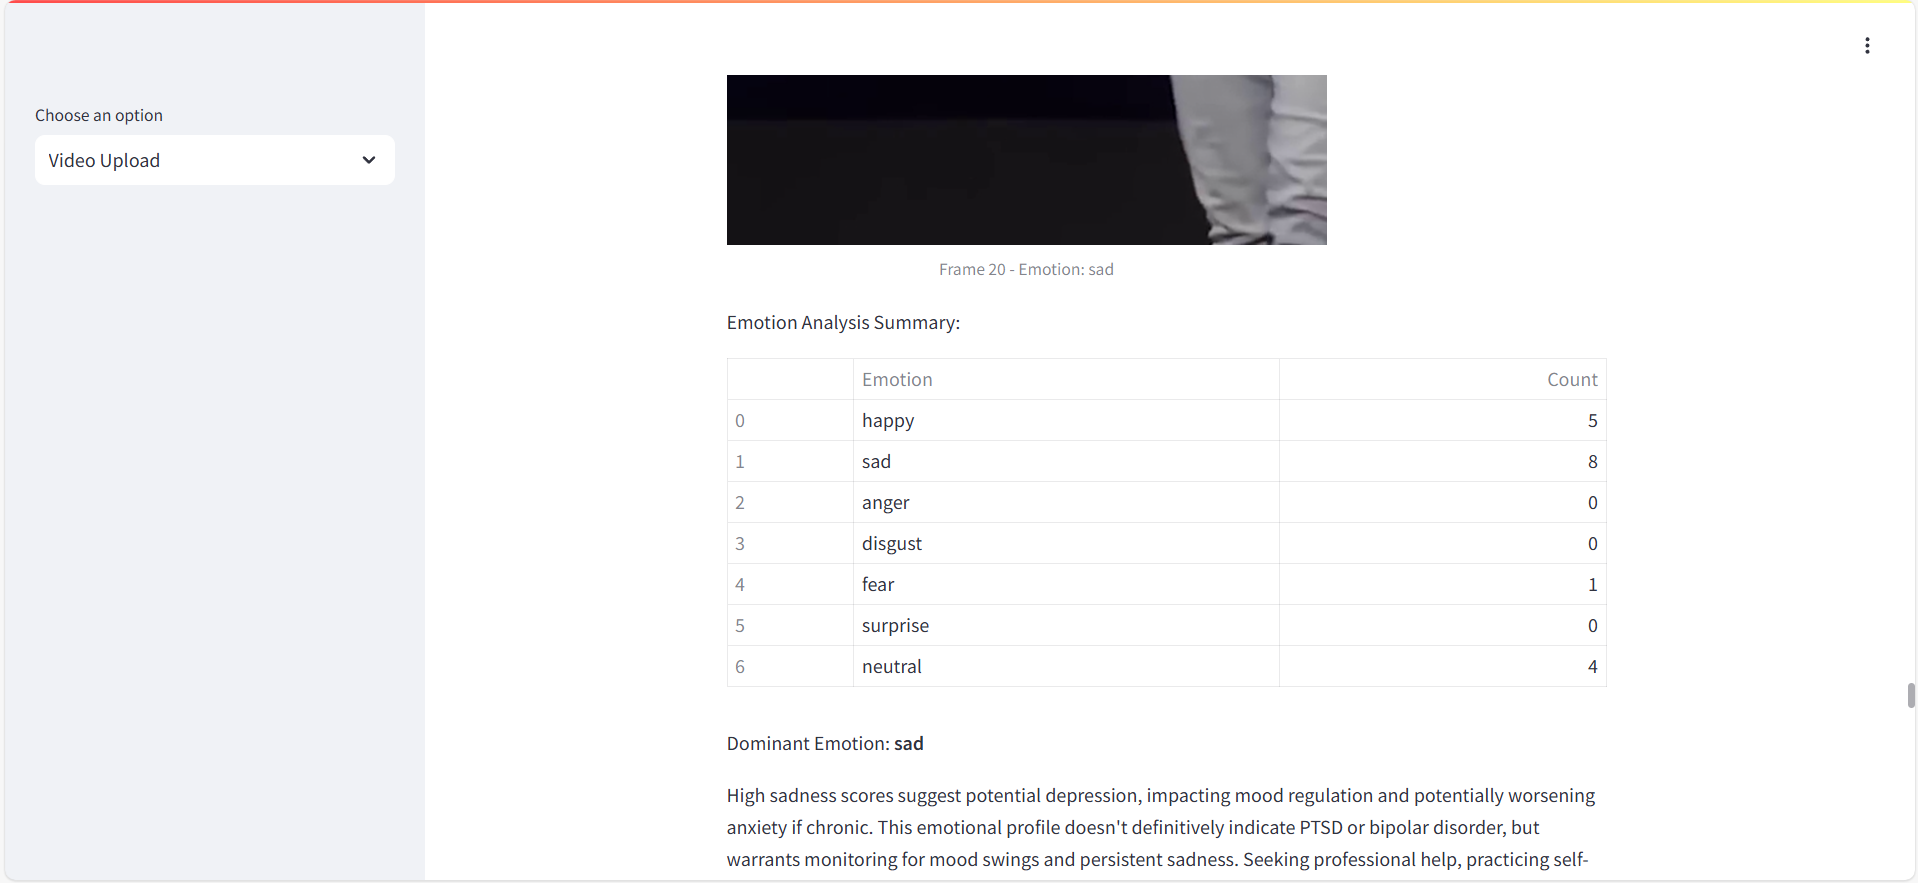
\includegraphics[width=1.0\textwidth]{App Images/12-1 Interface.png}  
    \caption{Result from the emotion analysis of facial expression}
    \label{10i23}  % Label for referencing the figure
\end{figure}


\pagebreak

\begin{tcolorbox}[colback=gray!5!white, colframe=gray!80!black, boxrule=0.5pt, title=Image Captioning]
    \begin{lstlisting}[language=Python]
# Function to load the model (cached for efficiency)
@st.cache_resource
def load_model():
    model_name = "nlpconnect/vit-gpt2-image-captioning"
    model = VisionEncoderDecoderModel.from_pretrained(model_name)
    feature_extractor = ViTImageProcessor.from_pretrained(model_name)
    tokenizer = AutoTokenizer.from_pretrained(model_name)
    return model, feature_extractor, tokenizer

# Load the model
IDmodel, IDfeature_extractor, IDtokenizer = load_model()

# Set device to GPU if available
device = torch.device("cuda" if torch.cuda.is_available() else "cpu")
IDmodel.to(device)

# Function to generate caption
def generate_caption(image):
    # Preprocess the image
    if image.mode != "RGB":
        image = image.convert(mode="RGB")
    pixel_values = IDfeature_extractor(images=image, return_tensors="pt").pixel_values
    pixel_values = pixel_values.to(device)

    # Generate caption (you can adjust max_length and num_beams as needed)
    with torch.no_grad():
        output_ids = IDmodel.generate(pixel_values, max_length=16, num_beams=4)
    caption = IDtokenizer.decode(output_ids[0], skip_special_tokens=True)
    return caption
\end{lstlisting}
    \end{tcolorbox}

\noindent
The provided code implements two key functionalities: image captioning and mental health text classification. For image captioning, it loads a pre-trained VisionEncoderDecoder model (vit-gpt2-image-captioning) using Hugging Face tools, processes input images, and generates captions. The \textbf{vit-gpt2-image-captioning} model combines two advanced architectures, the Vision Transformer (ViT) and GPT-2, to generate descriptive captions for images. It functions as an encoder-decoder system where ViT acts as the encoder to process and extract meaningful features from the image, and GPT-2 acts as the decoder to generate coherent natural language captions based on those features. The Vision Transformer (ViT) is a transformer-based model for image recognition. Unlike traditional convolutional neural networks (CNNs), which process images in a grid-like fashion, ViT splits the image into smaller patches (e.g., 16x16 pixels). These patches are flattened into vectors and passed through a transformer encoder. This encoder treats each patch as a token, similar to how words are tokens in natural language processing. By leveraging self-attention mechanisms, ViT captures both local and global dependencies in the image, resulting in a comprehensive feature representation. These features are passed to the decoder for further processing. GPT-2, a pre-trained generative language model, serves as the decoder. It uses the features extracted by ViT to generate captions word by word. Transformers like GPT-2 rely heavily on self-attention and positional encodings to understand the relationships between words in a sequence. In this context, GPT-2 uses the visual feature embeddings as the initial context and generates text sequentially. At each step, it predicts the next word in the caption based on the previous words and the image features, ensuring that the captions are contextually relevant and grammatically accurate. Transformers are crucial here because they allow the model to handle complex dependencies and interactions in both image and text data. ViT uses transformers to learn rich visual representations by modeling relationships between patches in the image, while GPT-2 leverages transformers to generate fluent and coherent text based on the encoded image features.
    

\begin{figure}[h!]  
    \centering
    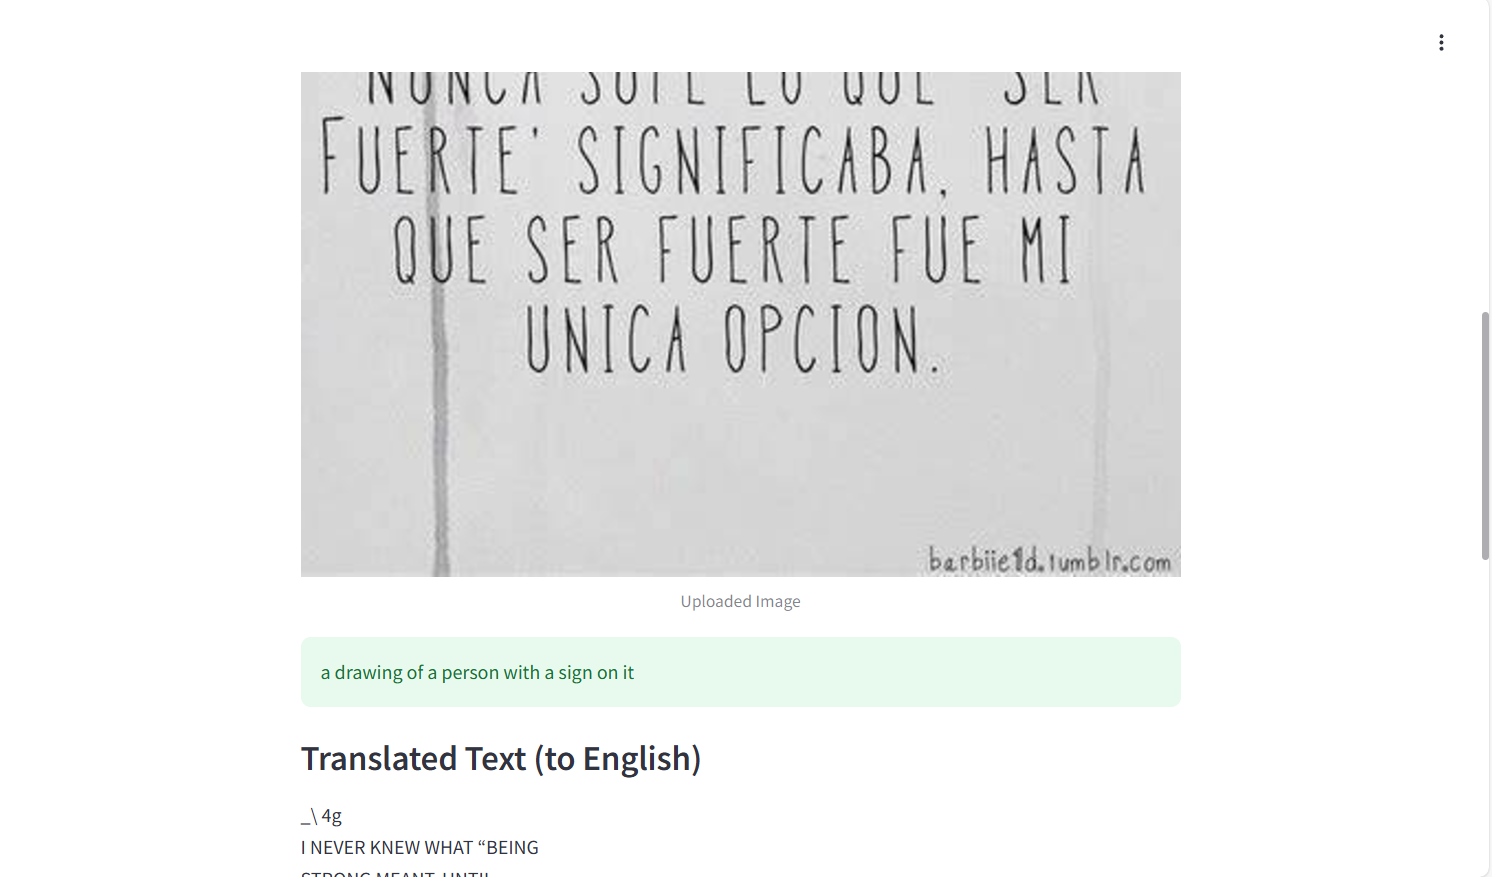
\includegraphics[width=1.0\textwidth]{App Images/18 Interface.png}  
    \caption{Generate Image Caption}
    \label{10i234}  % Label for referencing the figure
\end{figure}   

% ---------- knowledge graph

\begin{tcolorbox}[colback=gray!5!white, colframe=gray!80!black, boxrule=0.5pt, title=Knowledge Graph Creation]
    \begin{lstlisting}[language=Python]
def create_knowledge_graph(input_text, classifications, probabilities):
    # Initialize a directed graph
    graph = nx.DiGraph()
    # Add the central node (input text)
    graph.add_node("Input Text", size=1500, color="#ADD8E6")  # Light blue for the central node
    # Normalize probabilities for better edge length scaling
    max_prob = max(probabilities)
    min_prob = min(probabilities)
    prob_scaled = [(1 - (p - min_prob) / (max_prob - min_prob)) + 0.1 for p in probabilities]  # Invert probabilities for distances

    # Add nodes for classifications and connect them to the input text
    for classification, probability, scaled_prob in zip(classifications, probabilities, prob_scaled):
        prob_percentage = f"{probability * 100:.2f}%"
        graph.add_node(classification, size=1000, color="#E6E6FA")  # Light lavender for classification nodes
        graph.add_edge("Input Text", classification, weight=scaled_prob, label=prob_percentage)

    # Extract node colors and sizes
    node_colors = [data["color"] for _, data in graph.nodes(data=True)]
    node_sizes = [data["size"] for _, data in graph.nodes(data=True)]
    # Compute positions using spring layout, scaling edge lengths with inverted probabilities
    pos = nx.spring_layout(graph, seed=42, weight='weight')

    # Draw the graph
    plt.figure(figsize=(12, 8))
    nx.draw(
        graph, pos, with_labels=True, node_size=node_sizes, node_color=node_colors,
        font_size=10, font_weight="bold", edge_color="gray")

    # Add edge labels for probabilities
    edge_labels = nx.get_edge_attributes(graph, "label")
    nx.draw_networkx_edge_labels(graph, pos, edge_labels=edge_labels, font_color="red")
    # Display the plot in Streamlit
    st.pyplot(plt)
    \end{lstlisting}
\end{tcolorbox}

\noindent
This code defines a function to create a knowledge graph that visualizes the relationships between an input text and mental health classifications along with their associated probabilities. It uses the NetworkX library to construct a directed graph, where the input text forms the central node connected to classification nodes, each representing a mental health issue. Probabilities are used to determine edge lengths dynamically, ensuring that classifications with higher probabilities are closer to the central node. The Matplotlib library is used to render the graph, with color-coded nodes for improved readability. The final visualization is displayed within a Streamlit application, allowing interactive exploration of the graph.


\begin{figure}[h!]  
    \centering
    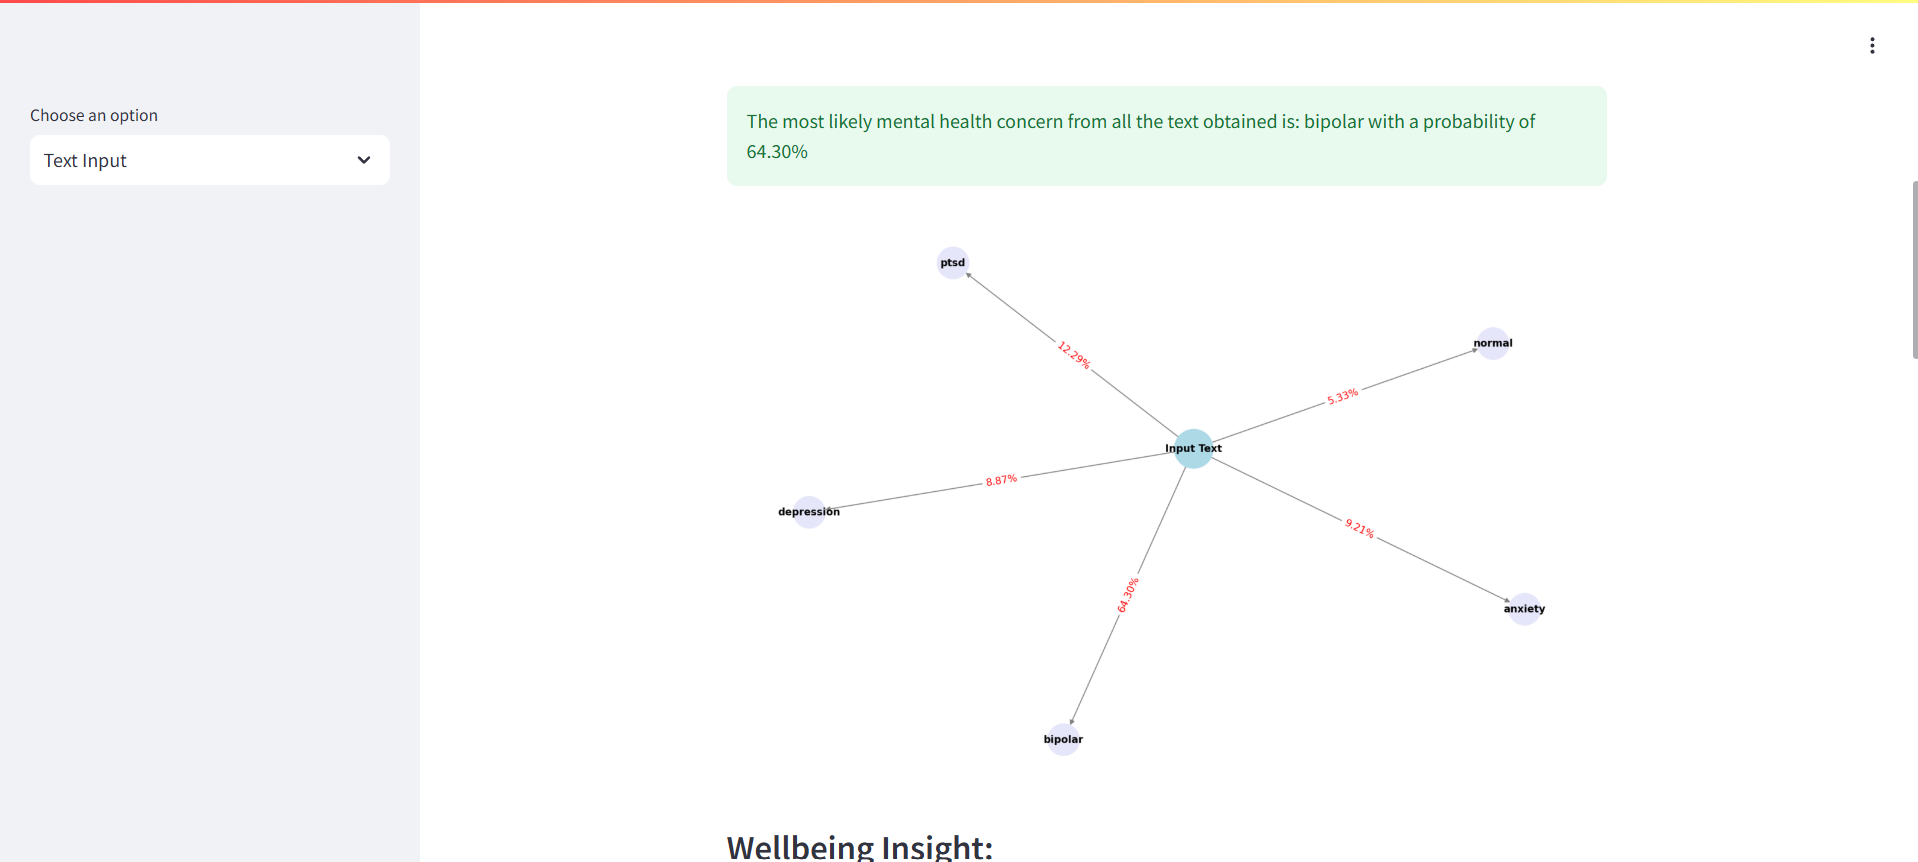
\includegraphics[width=1.0\textwidth]{App Images/19 Interface.png}  
    \caption{Knowledge Graph from classification}
    \label{10i23445}  % Label for referencing the figure
\end{figure}  


% ----------------------- Prototype ends -------------------


\begin{comment}

    \section*{APPENDIX B - Paper publications (optional) \label{sec:pubs}}
\addcontentsline{toc}{section}{APPENDIX B - Paper publications (optional)}
If any of your related paper(s) were published in a standard journal / presented in a recognized conference, mention the same including communication on your paper(s) acceptance / publishing note. You should also show appropriate documentation at the time of project viva.


\end{comment}

